\documentclass[12pt,a4paper]{article}
\usepackage[utf8]{inputenc}
\usepackage{amsmath}
\usepackage{amsfonts}
\usepackage{enumitem}
\usepackage{amssymb}
\usepackage{graphicx}
\usepackage{amsthm}
\author{Marco Bertenghi}


\usepackage{color}  
\usepackage{hyperref}
\hypersetup{
    colorlinks=true, %set true if you want colored links
    linktoc=all,     %set to all if you want both sections and subsections linked
    linkcolor=blue,  %choose some color if you want links to stand out
}
\newtheorem{lem}{Lemma}[section]
\newtheorem{thm}{Theorem}[section]
\newtheorem{prop}{Proposition}[section]
\newtheorem{cor}{Corollary}[section]
\newtheorem{defn}{Definition}[section]
\newtheorem{exmp}{Example}[section]
\theoremstyle{definition}
\newtheorem{rem}{Remark}[section]

\title{Graph Theory}
\date{}

\begin{document}
\begin{titlepage}
	\centering
	
	{\scshape\LARGE University of Zurich \par}
	\vspace{2cm}
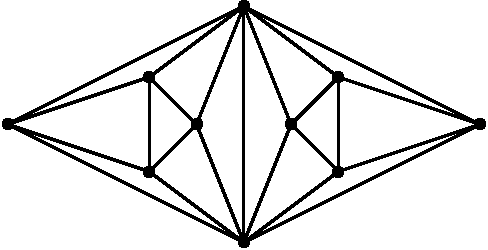
\includegraphics[width=.8\textwidth]{logo1.pdf}\par\vspace{1cm}
	\vspace{1cm}
	{\huge\bfseries Graph Theory\par}
	\vspace{2cm}
	{\Large\itshape Prof. Dr. Ashkan Nikeghbali\par}
	\vfill
	\LaTeX \ by\par
	Marco \textsc{Bertenghi}

	\vfill

% Bottom of the page
	{\large \today\par}
\end{titlepage}
\newpage
\thispagestyle{empty}
\tableofcontents
\newpage
\maketitle
\begin{figure}[hbtp]
\centering
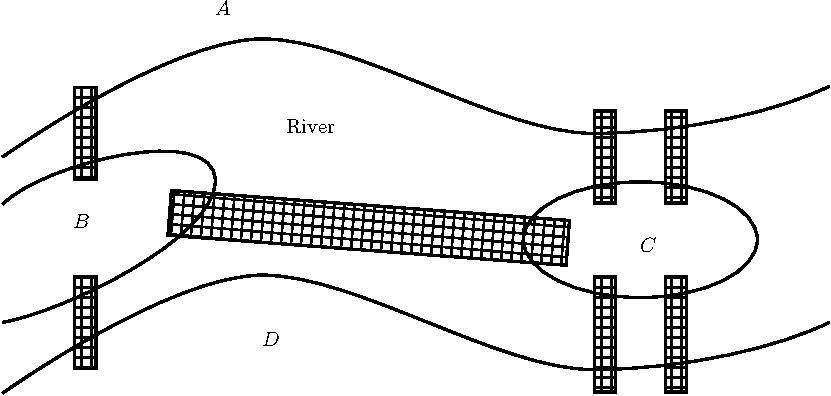
\includegraphics[scale=.7]{images/koenigsberger.pdf}
\caption{Königsberg's bridge problem}
\end{figure}
Königsberg's bridges problem: Is it possible to walk through town,  starting and ending at the same point, so that we use each bridge exactly once? This problem, solved by Euler, is considered as the starting point of graph theory. 
\section{Basic concepts}
\begin{defn} A \textbf{graph} $G$ is a pair $G=(V(G),E(G))$, or more simply $G=(V,E)$ where $V$ is a finite set and $E$ is a finite set, possibly empty, endowed with an application $f: E \to P_2(V) \cup P_1(V)$ where $P_2(V)$ denotes all subsets of $V$ with two elements, and $P_1(V)$ all subsets containing only a single element of $V$. The elements of $V$ are called \textbf{vertices}, the elements of $E$ are called \textbf{edges}. The cardinality of $V$ is called the \textbf{order} of $G$. The \textbf{size} of the graph is the cardinality of the edge set $E$. For $f(e)= \{u,v\}$, we say that $u$ and $v$ are \textbf{endvertices} of $e$ and that the vertices $u$ and $v$ are \textbf{adjacent}. A \textbf{loop} is an edge $e$ such that $f(e) \in P_1(V).$ If $f^{-1}(\{u,v\})$ is of cardinality $1$, then we say that $f^{-1}(\{u,v\})$ is a \textbf{simple edge}. If $f^{-1}(\{u,v\})$ is of cardinality $\geq 2$,then we say that $f^{-1}(\{u,v\})$ is a \textbf{multiple edge}. A vertex which is the endpoint of no edge is called \textbf{isolated}. 
\end{defn}
\newpage
\begin{exmp} \
\begin{figure}[hbtp]
\centering
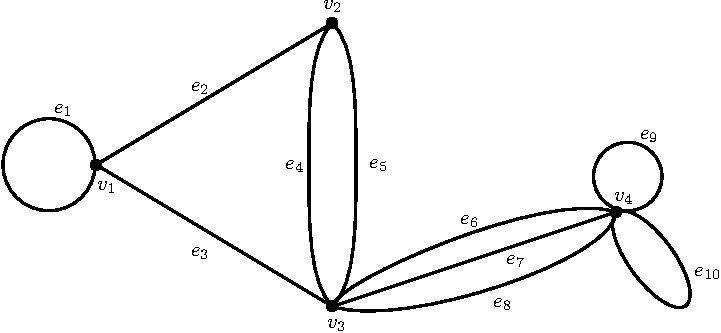
\includegraphics[scale=1]{images/graph1.pdf}
\caption{$V=\{v_1,v_2,v_3,v_4,v_5\}$, $E=\{e_1,e_2,e_3,\dots,e_{10}\}$}
\end{figure} \\
$f(e_1)=\{v_1\}, \ f(e_2)= \{v_1,v_2\}, \ f(e_3)= \{v_1,v_3\}, \ f(e_4)= f(e_5)= \{v_2,v_3\}$, $f(e_6)=f(e_7)=f(e_8)=\{v_4,v_4\}$, $f(e_9=f(e_{10}) = \{v_4\}$. $e_2$ and $e_3$ are simple edges. $\{e_4,e_9\}$ and $\{e_6,e_7,e_8\}$ are multiple edges. $e_1$ is a simple loop. $\{e_9, e_{10}\}$ are multiple loops. $v_5$ is an isolated vertex. 
\end{exmp}
\begin{defn} A graph $G=(V;E)$ is called \textbf{simple} if it has no loops and no multiple edges. In this case, if $E \neq \emptyset$, $f: E \to P_2(V)$ is an injection and we identify $e$ with $f(e)$. For notational convenience, instead of representing an edge as $\{u,v\}$, we denote it by $uv$. 
\end{defn}
\begin{rem} \
\begin{enumerate}
\item  In a simple graph $G$ with $n$ vertices and $m$ edges, we have 
\begin{align*}
m \leq \ { n \choose 2} = \frac{n(n-1)}{2}.
\end{align*}
\item In the literature, and in what follows, a simple graph is simply called a graph. Then a graph with multiple edges is called a \textbf{multigraph} and a graph with loops is called a \textbf{pseudograph}.
\end{enumerate}
\end{rem}
If in a graph we decide that the order of the vertices matters, then we make the following definition:
\begin{defn} A \textbf{directed graph} (or \textbf{digraph}) is a pair $G=(V(G),A(G))$ or more simply $G=(V;,A)$ where $V$ is a non empty finite set and where $A$ is a set, possibly empty, endowed with an application $f: A \to V \times V$.
\end{defn}
This time we have $f(a)=(u,v)$ which is in general different from $(v,u)$. A directed graph is usually represented as follows: 
\newpage
\begin{figure}[hbtp]
\centering
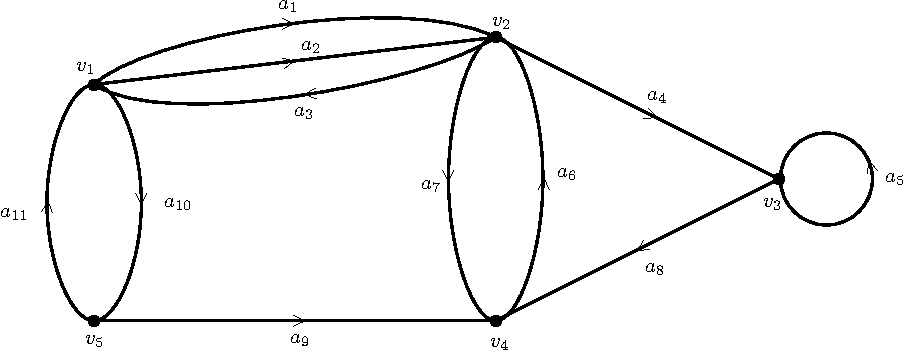
\includegraphics[scale=.8]{images/graph3.pdf}
\caption{A directed graph.}
\end{figure}
\begin{rem}Allowing edges to be arbitrary subsets of vertices (rather then just singletons or pairs) gives us a \textbf{hypergraph}:
\begin{figure}[hbtp]
\centering
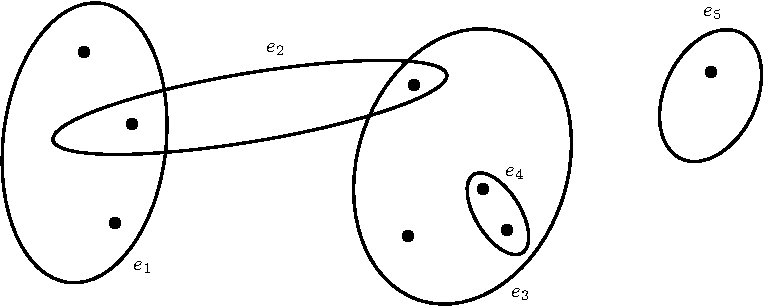
\includegraphics[scale=.8]{images/graph4.pdf}
\caption{A hypergraph.}
\end{figure}

\end{rem}
\begin{defn} The \textbf{neighborhood} of a vertex $v$, denoted by $N(v)$, is the set of vertices adjacent to $v$: $N(V)= \{ x \in V, vx \in E\}.$ The \textbf{closed neighborhood} of a vertex $v$, denoted by $N[v]$, is teh set $\{v\} \cup N(v)$. Given a set $S$, we define the neighborhood of $S$, denoted by $N(S)$, to be the union of neighborhoods of the vertices in $S$, i.e. $N(S):= \bigcup_{v \in S} N(v)$. Similarly we define the closed neighborhood of $S$, denoted by $N[S]$, as $S \cup N(S)$. The \textbf{degree} of $v$, denoted by deg$(v)$ or $d(v)$, is the number of edges incident with $v$. In simple graphs we have $d(v)= |N[v]|$. The \textbf{maximum degree} of a graph $G$, denoted by $\Delta(G)$, or $\Delta$, is defined as $\Delta(G)= \max \{ d(v), v \in V(g)\}.$ Similarly the \textbf{minimum degree} of a graph $G$, denoted by $\delta(G)$, is defined as $\delta(G)= \min \{ d(v), v \in V(G) \}.$ The \textbf{degree sequence} of a graph $G$ of order $n$ is the $n$-term sequence (usually written in increasing order) of the vertex degrees. 
\end{defn}
\newpage
\begin{exmp} \
\begin{figure}[hbtp]
\centering
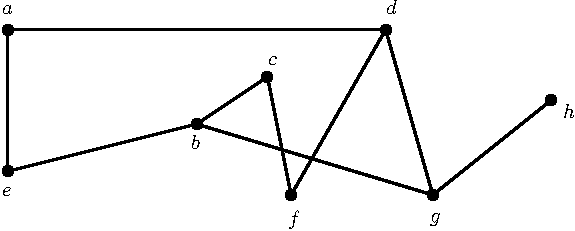
\includegraphics[scale=1]{images/graph5.pdf}
\end{figure}
\\
$N(d)= \{a,fg\}, \ N[d] = \{a,d,f,g\}, \ \Delta(g)=3, \ \delta(G)=1$. Degree sequence: $(1,2,2,2,2,3,3,3)$.
\end{exmp}
\begin{thm} In a (loopless) graph, the sum of the degrees of the vertices is equal to twice the number of edges. Consequently the number of vertices with odd degree is even. 
\end{thm}
\begin{proof}
In $\sum_{v \in V} d(v)$, we count each edge exactly twice. This entails that  $\sum_{v \in V} d(v) = 2 |E|$.
\end{proof}
\begin{defn} A sequence $D=(d_1, \dots , d_n)$ with $d_1 \leq d_2 \leq \dots \leq d_n$, is called \textbf{graphical} if there exists a graph $G$ on $n$ vertices such that $D$ is its degree sequence. 
\end{defn}
\begin{thm} Let $n$ be an integer $\geq 1$. Let $D=(d_1, \dots , d_n)$ be a sequence of integers such that $d_1 \leq d_2 \leq \dots \leq d_n$. There exists a graph $G$ on $n$ vertices such that $D$ is its degree sequence iff the sequence $D'=(d_1', \dots , d_{n-1}')$ defined by
\begin{align*}
d_i' = \begin{cases} d_i, & \text{ if } 1 \leq i < n -d_n \\ d_i-1, & \text{ otherwise}\end{cases}
\end{align*}
is a graphical sequence. 
\end{thm}
\begin{proof}
($\Leftarrow$) Let $D=(d_1, \dots , d_n)$ be such that $D'$ is a graphical sequence. Then there exists a graph $G'$ on $n-1$ vertices such that $D'$ is its degree sequence. Let us add a vertex  $v$ to $G'$, adjacent to the vertices of degree $d_{n-d_n} -1, \dots , d_{n-1}-1$. Thus the degree sequence of $G$ is $(d_1', \dots , d_{n-d_{n-1}}', \dots , d_{n-1}, d_n)= (d_1, \dots , d_n)$. 
\\\\
($\implies$) Let $G=(V,E)$ be a graph with degree sequence $D=(d_1, \dots , d_n)$. Note that $d_n$ is the maximal degree of $G$. Let $w$ be a vertex of $G$ such that $d(w)=d_n = \Delta$. Let $S$ be the set of $n$ vertices of degree $d_{n-d_n}, \dots , d_n$. If $N(w)=S$, then we can remove $w$ and its adjacent edges and we obtain a graph $G'$ whose degree sequence is $D'$. Let us assume that $N(w) \neq S$. As $|N(w)| = |S|$, there exists $x \in S \setminus N( w)$ and $\eta \in N(w) \setminus S$. It follows from the choice of $S$ that $d(x) \geq d( \eta)$. Let us now note that there is a vertex $y \notin \{ x,  \eta, w \}$ such that $ y$ is adjacent to $x$, but not to $\eta$. Indeed, the number of neighbors of $x$, excluding $\eta$, is $d(x)= \epsilon$ where $\epsilon = 1$ if $x$ is adjacent to $\eta$ and $0$ otherwise. The number of neighbors of $\eta$ other than $x$ and $w$ is $d( \eta)=1- \epsilon$. Note that we have the existence of $y$ because $d(x) \geq d( \eta)$. 
\begin{figure}[hbtp]
\centering
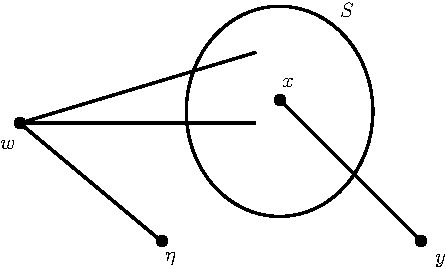
\includegraphics[scale=1]{images/graphmiss.pdf}
\end{figure}
\\
We then consider the graph $G_1=(V,E \setminus \{ \{w, \eta\}, \{x, y\} \} \cup \{ \{ w,x\}, \{ \eta, y\} \})$. We haven't changed the degree sequence but increased by $1$ $|N(w) \cap S|$. Continuing this process, we obtain a graph with degree sequence $D$ and $N(w) = S$. 
\end{proof}
\begin{exmp} Prove that $(1,1,1,2,2,2,3,3,3)$ is a graphical sequence. Let us apply the previous theorem. 
\begin{align*}
&\rightarrow (1,1,1,2,2,1,2,2)  & \quad \text{that we rewrite}   & \qquad (1,1,1,1,2,2,2,2). \\
&\rightarrow (1,1,1,1,2,1,1)  & \text{that we rewrite}  & \qquad (1,1,1,1,1,2). \\
& \rightarrow (1,1,1,1,0,0) & \text{that we rewrite} & \qquad (0,0,1,1,1,1). \\
 & \rightarrow (0,0,1,1,0) 
\end{align*}
where $(0,0,1,1,0)$ is simply the degree sequence of the empty graph on $3$ vertices or a path on $2$ vertices.
\end{exmp}
We now wish to introduce the concept of graph isomorphism. For this we introduce a few more definitions. 
\begin{defn} Pairwise non-adjacent vertices or edges are called \textbf{independent}. More generally a set of vertices or edges is independent if no two of its elements are adjacent. Independent sets of vertices are also called \textbf{stable}.
\end{defn}
\begin{defn} Let $G=(V,E)$ and $G'=(V',E')$ be two (simple) graphs. A map $f : V \to V'$ is a \textbf{homomorphism} from $G$ to $G'$ if it preserves the adjacency of vertices, that is $\{x,y\} \in E \to \{ f(x), f(y)\} \in E'$. Then in particular for every $x' \in f(V)$, $f^{-1}( \{x'\})$ is an independent set of vertices in $G$. If $\varphi$ is bijective and its inverse $f^{-1}$ is also a homomorphisms, so that for all $x,y \in V$ we have $xy \in E \iff f(x) f(y) \in E'$, then we call $f$ an \textbf{isomorphisms}, we say that $G$ and $G'$ are \textbf{isomorphic}, and write $G \simeq G'$. An isomorphism from $G$ to itself is an \textbf{automorphism} of $G$. In general we do not distinguish between isomorphic graphs. 
\end{defn}
\begin{rem} A class of graphs that are closed under isomorphisms is called a \textbf{graph property}. For example "containing a triangle" is a graph property. Indeed if $G$ contains three pairwise adjacent vertices then so does every graph isomorphic to $G$.
\end{rem}
\begin{defn} A map taking graphs as arguments is called a \textbf{graph invariant} if it assigns equal values to isomorphic graphs. The number of vertices and the number of edges of a graph are two simple graph invariants. The degree sequence is another one. 
\end{defn}
Let us illustrate the above with examples. 
\begin{figure}[hbtp]
\centering
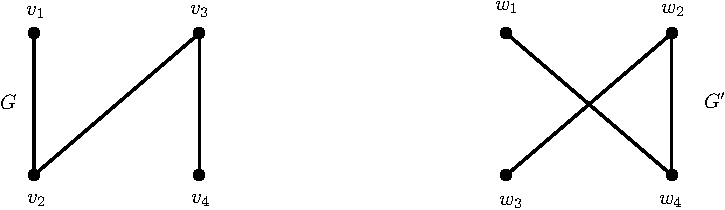
\includegraphics[scale=1]{images/graph7.pdf}
\caption{$G \simeq G'$, $f(v_1)=w_1, f(v_2)=w_4, f(v_3)=w_2, f(v_4)=w_3$.}
\end{figure}
\begin{figure}[hbtp]
\centering
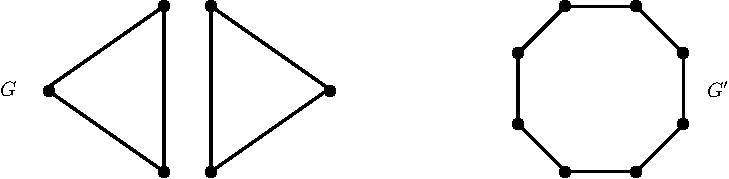
\includegraphics[scale=1]{images/graph8.pdf}
\caption{$G$ and $G'$ are not isomorphic.}
\end{figure}
\\
$G$ and $G'$ are not isomorphic even though $|V(G)|=|V(G')|$ and $|E(G)|=|E(G')|$, and the degree sequence for both graphs is $(2,2,2,2,2,2)$.
\newpage
\section{Special graphs}
\subsection{Complete graphs}
A graph is said to be complete if every vertex is adjacent to every other vertex. A complete graph on $n$ vertices is denoted by $K_n$, and sometimes called a $n$-clique.
\begin{figure}[hbtp]
\centering
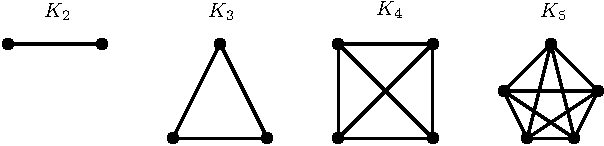
\includegraphics[scale=1]{images/graph9.pdf}
\caption{The figures above depict the complete graphs $K_2, \dots , K_5$.}
\end{figure}
\subsection{Empty graphs}
The empty graph on $n$ vertices, denoted by $E_n$, is the graph of order $n$ where $E$ is the empty set.
\begin{figure}[hbtp]
\centering
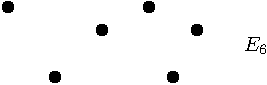
\includegraphics[scale=.8]{images/graph10.pdf}
\caption{Empty graph on $6$ vertices.}
\end{figure}
\subsection{Complements}
Given a graph $G$, the complement of $G$,  denoted by $\overline{G}$, is the graph whose vertex set is the same as that of $G$, and whose edge set consists of all the edges that are \textbf{not} in $G$.
\begin{figure}[hbtp]
\centering
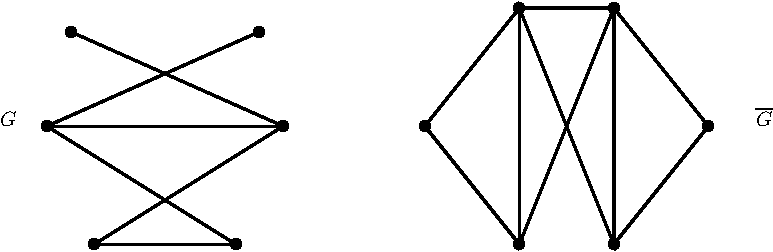
\includegraphics[scale=.7]{images/graph11.pdf}
\caption{$G$ and its complement $\overline{G}$.}
\end{figure}
\newpage
\subsection{Regular graphs}
A graph $G$ is regular if every vertex has the same degree. $G$ is said to be regular of degree $r$ or $r$-regular  if $d(v)=r$ for all $v \in V(G)$. Complete graphs are regular of degree $n-1$, and empty graphs are regular of degree $0$.
 \begin{figure}[hbtp]
\centering
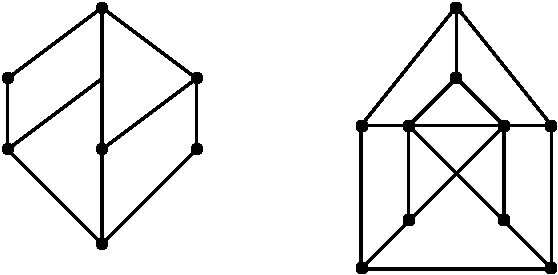
\includegraphics[scale=.7]{images/graph12.pdf}
\caption{The picture on the right is a $3$-regular Petarsen graph.}
\end{figure}\\
Since $\sum_{v \in V(G)} d(v)=2 |E|$, we have $k|V|=kn=2|E|$ So both $r$ and $n$ cannot be odd.
\begin{thm} Let $r$ and $n$ be integers,  such that $0 \leq r \leq n-1$. Then there exists an $r$-regular graph of order $n$ iff at least one of the integers $r$ or $n$ is even. 
\end{thm}
\begin{proof}
Let $r$ and $n$ be given, $0 \leq r \leq n-1$, such that one of them is even. We are going to construct a graph $H_{n,r}$ of order $n$ which is $r$-regular. Let us enumerate the vertices of $H_{n,r}$ as $v_0,  \dots , v_{n-1}$ and let us put them in order on a circle. If $r$ is even, we note $r=2k$ for some integer $k$. For each vertex $v_i$, we draw an edge with $v_{i+2}, \dots , v_{i+k}$ and $v_{i-k}, \dots , v_{i-k}$ ($i+1,…,i+k,i-1,…i-k$ are defined modulo $n$). $H_{n,r}$ is then $r$-regular. Now let us assume that $r$ is odd, and $n$ is even. Let $r=2k-1$ and $n=2l$. As before, we draw an edge between the $k$ following vertices as well as the $k$ preceding vertices, and fraw an additional edge to $v_{i+l}$. The graph $H_{n,r}$ obtained this way is $r$-regular.
\begin{figure}[hbtp]
\centering
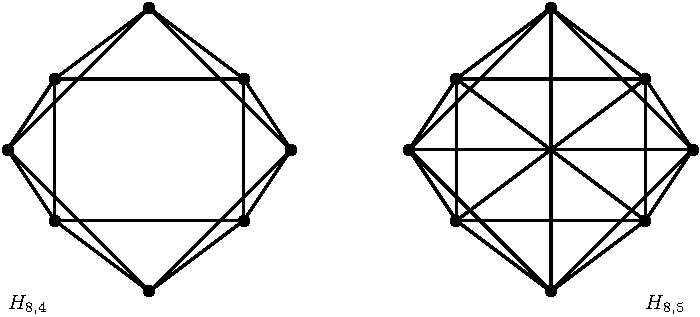
\includegraphics[scale=.72]{images/haraysgraph.pdf}
\caption{The Haray's graphs $H_{8,4}$ and $H_{8,5}$.}
\end{figure}

\end{proof}
\newpage
\subsection{Cycles}
For $n \geq 3$, the $n$-cycle, noted $C_n$ is the (simple) graph of order $n$ such that $V(C_n)=\{v_1, \dots ,  v_n\}$ and $E(C_n)= \{ \{v_i, v_{i+1} \}, i = 1, \dots ,  n-1 \} \cup \{ v_n, v_1 \}$. 
\begin{figure}[hbtp]
\centering
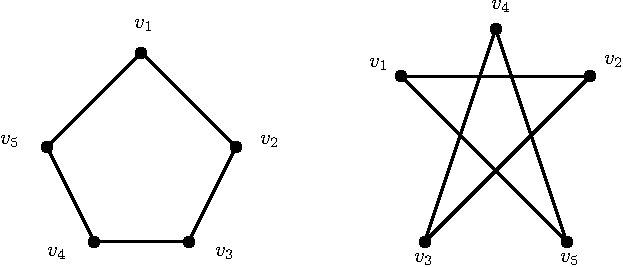
\includegraphics[scale=1]{images/graph13.pdf}
\caption{Cycles of order $5$.}
\end{figure}
\subsection{Paths} For $n \geq 1$, the graph $P_n$, called $n$-path, is the graph of order $n-1$ such that $V(P_n)= \{ v_0,  v_1, \dots , v_n \}, \ E(P_n)= \{ \{ v_i, v_{i+1}\} , i = 0, \dots , n-1 \}$. 
\begin{figure}[hbtp]
\centering
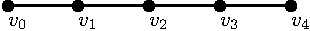
\includegraphics[scale=1]{images/graph14.pdf}
\caption{The path $P_4$.}
\end{figure}
\newpage
\subsection{Subgraphs}
A graph $H$ is a \textbf{subgraph} of $G$ if $V(H) \subset V(G)$ and $E(H) \subset E(G)$. in this case we write $H \subset G$ and we say that $G$ contains $H$. In a graph where vertices and edges are unlabelled, we say that $H \subset G$ if the vertices, could be labelled  in such a way that $V(H) \subset V(G)$ and $E(H) \subset E(G)$. 
\begin{figure}[hbtp]
\centering
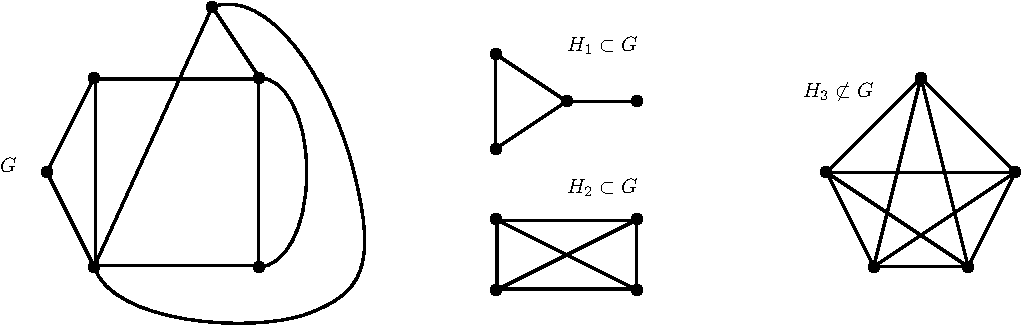
\includegraphics[scale=.8]{images/graph15.pdf}
\caption{The graph $G$ with its subgraphs $H_1, H_2$ and a non-subgraph $H_3$.}
\end{figure}
\subsection{Induced Subgraphs} Given a graph $G$ and a subset $S$ of the vertex set, the \textbf{subgraph of $G$ induced} by $S$, denoted by $\langle S \rangle$, is the subgraph with vertex set $S$ and with edge set $\{uv, u \in S, v \in S, uv \in E(G) \}.$ So $\langle S \rangle$ contains all vertices of $S$ and all edges of $G$ whose end vertices are both in $S$. Sometimes $\langle S \rangle$ is also denoted as $G[S]$. 
\begin{figure}[hbtp]
\centering
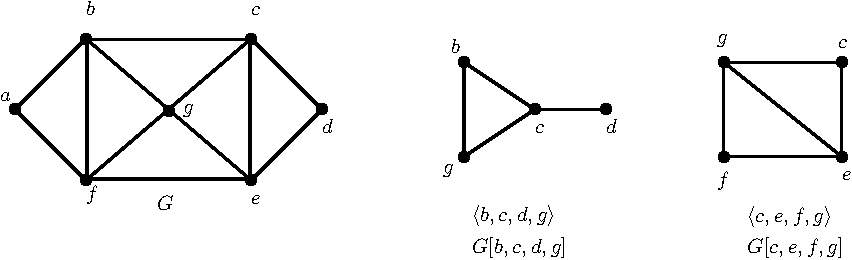
\includegraphics[scale=1]{images/graph16.pdf}
\caption{Example of induced subgraphs.}
\end{figure}
\newpage
\subsection{$k$-partite graphs}
Let $G=(V,E)$ be a graph of order $n$ and let $k \leq n$. The graph $G$ is called $k$-partite if there exists a partition of $V= V_1 \cup  \dots \cup V_k$ such that for every $1 \leq i \leq k$, $\langle V_i \rangle$ (or $G[V_i])$ is the empty graph. Such a graph is sometimes noted as $G=(V_1, \dots , V_k;E)$. When $k=2$, the graph is called \textbf{bipartite}. Note that if $G$ is $k$-partite, than it is also $h$-partite for $k \leq h \leq n$. 
\begin{figure}[hbtp]
\centering
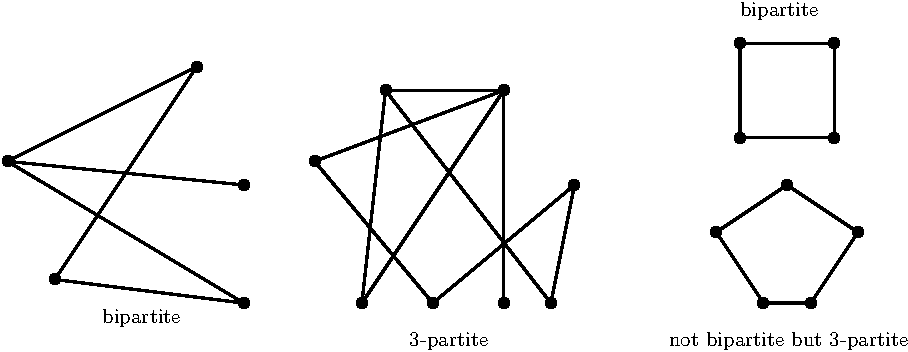
\includegraphics[scale=.9]{images/graph17.pdf}
\caption{Example of bipartite and $3$-partite graphs.}
\end{figure}
\\
A $k$-partite graph $G(V_1, \dots , V_k; E)$ is called complete $k$-partite graph if $\{xy\} \in E$ whenever $x \in V_i,  y \in V_j, i \neq j$. If for all $1 \leq i \leq k, |V_i| = n_i$, then we note the graph $K_{n_1, \dots , n_k}$.
\begin{exmp} \
\begin{figure}[hbtp]
\centering
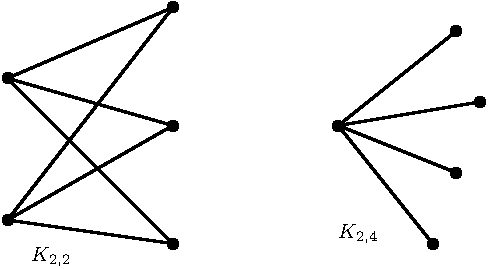
\includegraphics[scale=.9]{images/graph18.pdf}
\caption{Complete $k$-partite graphs}
\end{figure}
\end{exmp}
\newpage
\section{Connectivity}
We start this section with some fundamental definitions.
\begin{defn} A \textbf{walk} in a graph is a sequence of (not necessarily distinct) vertices $v_1, v_2, \dots , v_k$ such that $v_iv_{i+1} \in E$ for $i=1, \dots , k-1.$  If the vertices in a walk are distinct, then the walk is called a \textbf{path}. If the edges in a random walk are distinct, then the walk is called a \textbf{trail}. In this way, every path is a trail, but not every trail is a path. A \textbf{closed path} or \textbf{cycle} is a path $v_1, \dots ,  v_k$, $k \geq 3$, together with the edge $v_kv_1$. Similarly a trail that begins and ends at the same vertex is called a \textbf{closed trail}, or \textbf{circuit}. The \textbf{length} of a walk (or path, or trail, or cycle, or circuit) is its number of edges, counting repetitions. 
\end{defn}
\begin{exmp} \
\begin{figure}[hbtp]
\centering
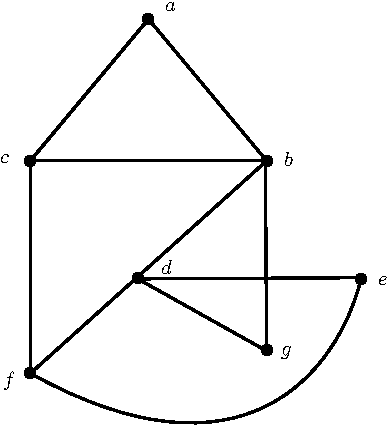
\includegraphics[scale=1]{images/graph19.pdf}
\caption{This figure is to help motivative the above fixed definitions.}
\end{figure}
\begin{itemize}
\item $a,c,f,c,b,d$ is  a walk of length $5$.
\item $b,a,c,b,a$ is a trail of length $4$.
\item $d,g,b,a,c,f$ is a path of length $5$.
\item $g,d,b,c,a,b,g$ is a circuit.
\item $e,d,b,a,c,f,e$ is a cycle.
\end{itemize}
\end{exmp}
\newpage
\begin{thm} In a simple graph, every $u-v$ walk contains a $u-v$ path ($u \neq v)$. 
\end{thm}
\begin{proof}[First proof] Let $W$ be a $u-v$ walk in $G$ with maximal length. Then $W$ is a path. Indeed, if this were not the case, and if $x$ is a vertex which is repeated twice, by removing the walk between $u$ and $x$ we would obtain a shorter walk which contradicts the fact that $W$ is of maximal length. 
\end{proof}
\begin{proof}[Second proof] Let $W$ be a $u-v$ walk. We prove this theorem by induction on the length of $W$. If $w$ is of length $1$ or $2$, then it is a path. \\
$<k \to k$. Say that $W$ is $u = w_0, w_1, \dots , w_{k-1}, w_k = v$. If the vertices are distinct, then $W$ itself is a $u-v$ path. If not, let $j$ be the smallest integer such that $w_j = w_r$ for some $r>j$. Let $W_j$ be the walk $u = w_0, w_1, \dots , w_j , w_{r+1}, \dots , w_k = v$. This walk has length $<k$ we can apply the induction assumption.

\end{proof}
\begin{cor} Let $G$ be a simple graph and let $u$ and $v$ be two distinct vertices of $G$. The following are equivalent:
\begin{enumerate}
\item There exists a $u-v$ walk in $G$.
\item There exists a $u-v$ in $G$.
\item There exists a $u-v$ path in $G$.  
\end{enumerate}
\end{cor}
\newpage
\begin{defn}
Given a graph $G$, and a vertex $v \in V(G)$, we let $G-v$ denote the graph obtained from $G$ by removing $v$ and all edges incident with $v$ in $G$.  If $S$ is a set of vertices, we let $G-S$ denote the graph, obtained by removing all vertices of $S$ and all associated incident edges of $G$. If $e$ is an edge of $G$, then $G-e$ is the graph obtained by removing only the edge $e$. If $T$ is a set of edges, then $G-T$ is the graph obtained by deleting each edge of $T$ from $G$. 
\end{defn}
\begin{figure}[hbtp]
\centering
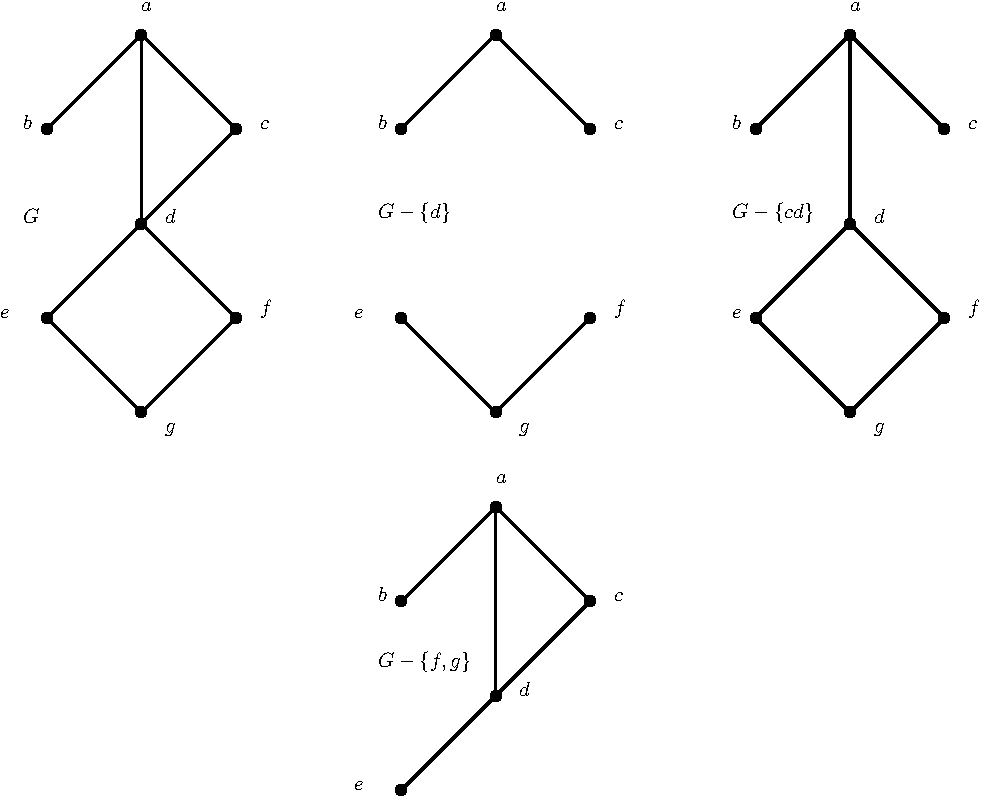
\includegraphics[scale=.85]{images/graph20.pdf}
\caption{Example motivating the above definitions.}
\end{figure}
\newpage
\begin{defn} A graph $G$ is \textbf{connected} if every pair of vertices can be joined by a path (or equivalently by a walk).
\end{defn}
\begin{prop} Let $G$ be a simple graph and let $\sim$ be the binary relation defined on $V(G)$ by $u \sim v$ iff there exists a $u-v$ walk in $G$. We then have
\begin{enumerate}
\item $\sim$ is an equivalence relation on $V(G)$.
\item  The equivalence classes of $V(G)$ form a partition of $V(G)$ and the obtained subgraphs by these equivalence classes are the connected components of $G$.
\item Every connected component is a connected graph.
\item The graph $G$ is connected iff it has a unique connected component.
\item If $G$ is not connected and if $u$ and $v$ are in two distinct connected components, then there exists a $u-v$ walk. 
\end{enumerate}
\end{prop}
\begin{prop} The vertices of a connected graph $G$ can always be enumerated, say $v_1, \dots , v_n$, so that $G_i = G[v_1, \dots , v_i]$ is connected for every $i=1, \dots , n.$
\end{prop}
\begin{proof}
Pick any vertex as $v_1,$ and assume inductively that $v_2, \dots ,  v_i$ have been chosen for some $i < |G|$. Now pick a vertex $v \in G- \{ v_1, \dots ,  v_i\}.$ As $G$ is connected, it contains a $u-v_1$ path $P$. Choose as $v_{i+1}$ the last vertex of $P$ in $G-\{v_1, \dots , v_i\},$ then $v_{i+1}$ has a neighbour in $G_i$. The results then follows by induction. 
\end{proof}
\begin{defn}If the deletion of a vertex $v$ from $G$ causes the number of connected components of $G$ to increase, then $v$ is called a \textbf{cut vertex}. In the example above (see Figure 19) $d$ is a cut vertex, whereas $c$ is not. Similarly an edge $e$ in $G$ is said to be a bridge if the graph $G-e$ has more components than $G$. In the example of Figure 19, $ab$ is the only bridge. A proper subset $S$ of vertices of a graph $G$ is called a \textbf{vertex cut} (or simply a \textbf{cutset}) if the graph $G-S$ is disconnected. 
\end{defn}
\begin{defn} Let $G=(V,E)$ be a (simple) graph. Let $A,B \subset V$ and let $X \subset V$ or $X \subset E $, $X \neq V$ or $X$ possibly empty. Assume that every $A-B$ path in $G$ contains a vertex or an edge from $X$. Then we say that $X$ \textbf{separates} the sets $A$ and $B$ in $G$. We say that $X$ separates two vertices $a$ and $b$ if it separates the sets $\{a\}, \{b\}$ but $a,b \notin X$. We say that $X$ separates $G$ if $X$ separates some two vertices in $G$. A separating set of vertices is called a \textbf{separator}.
\end{defn}
\newpage
\begin{defn} $G$ is called \textbf{$k$-connected} if $|G|>k$ and $G-X$ is connected for every set $X \subset V$ with $|X| <k$. In other words, no two vertices of $G$ are separated by strictly less than $k$ vertices. Equivalently, $G$ is $k$-connected iff every separator of $G$ has at least $k$-elements. Every graph is $0$-connected and the $1$-connected graphs are the non-trivial connected graphs. The greatest integer $K$ such that $G$ is $k$-connected is the \textbf{connectivity} $K(G)$ of $G$. If $|G| >1$ and $G-F$ is connected for every set $F \subset E$ of fewer than $\lambda$ edges, then $G$ is called \textbf{$\lambda$-edge-connected}. The greatest integer $\lambda$ such that $G$ is $\lambda$-edge-connected is the \textbf{edge connectivity} $\lambda(G)$ of $G$. In particular, $\lambda (G)=0$ iff $G$ is disconnected.
\end{defn}
\begin{rem} A $k$-connected graph is also $h$-connected for $h \leq k$. 
\end{rem}
\begin{exmp}\
\begin{figure}[hbtp]
\centering
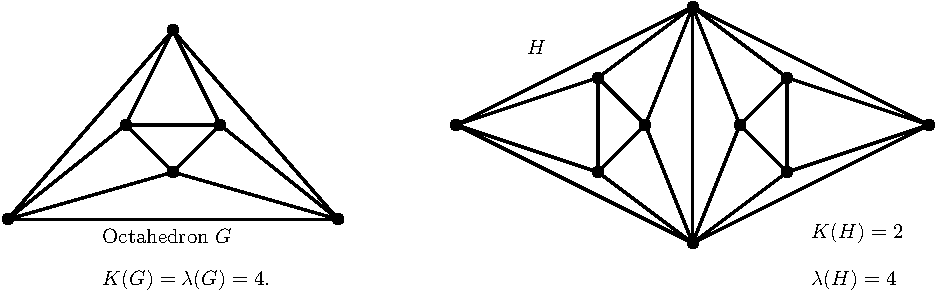
\includegraphics[scale=.8]{images/graph21.pdf}
\caption{Introducing the connectivity constants $K$ and $\lambda$.}
\end{figure}

\end{exmp}
\begin{lem} Let $G$ be a $k$-connected graph, with $k \geq 1$ and let $e \in E(G)$. Then the graph $G-\{e\}$ is $(k-1)$-connected.
\end{lem}
\begin{proof}
Note that $K(G-e) \leq K(G).$ If $K(G-e)=K(G)$, then the result is trivial. If $G=K_n$, then $K(G)=n-1$ and $K(G-e)=n-2=K(g)-1$ and the result follows again. Let us thus assume that $K(G-e) < K(G)$ and $G \neq K_n.$ Then $K(G) \leq n-2$ and $K(G-e) \leq n-3 $. Let $S$ be a not separating set of $G-e$ with minimal cardinality, which is not separating for $G$. The graph $G-e \setminus S$ is not connected and each vertex of $e$ belongs to different connected components of $G-e \setminus S$. But since $|S| \leq n-3$, then one of the connected components has at least an element $\eta \neq x, \eta \neq y$, where $e=xy$. Let us assume that $\eta$ and $x$ are in the same connected component. Then $S \cup \{x\}$ is separating $G$. Thus $K(G) \leq K(G \setminus \{e\}) +1$ so $K(G-e) \geq K(G)-1 \geq k-1$. 
\end{proof}
\newpage
\begin{prop} If $G$ is a graph of order $\geq 2$, then we have $K(G) \leq \lambda (G) \leq \delta(G)$. 
\end{prop}
\begin{proof}
The only non trivial inequality to prove is $K(G) \leq \lambda (G)$. If $G$ is not connected, then $K(G)= \lambda(G)=0$. Let $n \geq 2$. If $G=K_n$, then $K(G) = \lambda(G) = n-1$. Let us thus assume that $G$ is connected with $G \neq K_n$. Let $X$ be a minimal separating set of edges, $\lambda(G)= |X| \leq \delta (G) \leq n-2$. Since $X$ is minimal, $G-X$ has exactly two connected components, $G_1$ and $G_2$, and all edges from $X$ have one adjoint in $G_1$ and the other one in $G_2$. Let $k= |E(G_1)| \geq 1$ and $ n-k= |E(G_2)| \geq 1$. If every vertex of $G_1$ is adjacent to every vertex of $G_1$, then $|X|=k(n-k)=(k-1)(n-k-1)+n-1 \geq n-1$ which contradicts an  assumption that $|X| \leq n-2$. Hence there exists a vertex $u \in V(G_1), v   \in V(G_2)$ which are not adjacent. Let $T$ be the set consisting of neighbours of $u$ in $G_2$ and all vertices in $G_1$ which has a neighbour in $G_1$. There is no $u-v$ walk in $G \setminus T$ by construction. Hence $T$ is a separator of $G$. Thus $K(G) \leq |T| \leq |X| = \lambda(G)$. 
\end{proof}
\begin{exmp} The previous inequalities can be strict as shown in the following example:
\begin{figure}[hbtp]
\centering
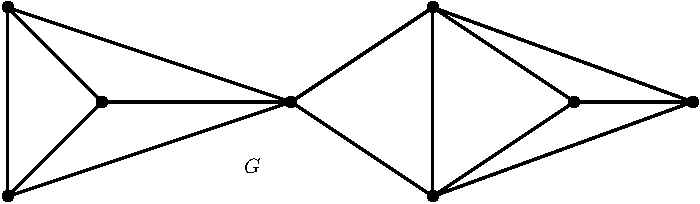
\includegraphics[scale=1]{images/graph22.pdf}
\caption{$H$ is $1$-connected with $K(G)=1$, $\lambda(G)=2$ and $\delta(G)=3$.}
\end{figure}

\end{exmp}
\begin{defn} We say that two $(u-v)$-walks are \textbf{internally disjoint} if $u$ and $v$ are the only common vertices of the two walks. If $W \subset V(G)$ separates the vertices $u$ and $v$, then two $(u-v)$-walks which are internally disjoint intersect $W$ at a distinct vertices. Thus the number of $(u,v)$-walks that are internally disjoint is at most $|W|$. 
\end{defn}
\begin{thm}[Menger] Let $u$ and $v$ be two distinct and non adjacent vertices of a simple graph $G$. Then the minimal cardinality of a set of vertices that separates $u$ and $v$ is equal to the maximum number of internally disjoint $(u,v)$-walks.
\end{thm}
\newpage
\begin{cor}[Whitney] Let $G$ be a simple graph, $|G| \geq 2$. The graph $G$ is $k$-connected iff any two vertices of $G$ can be formed by at least $k$ walks which are internally disjoint. In particular, the graph $G$ is $2$-connected iff two arbitrary vertices of $G$ belong to the same cycle. 
\end{cor}
\begin{proof}
 For $k=1$ the result is immediate. Let us assume $k \geq 1$. \\\\
 "$\implies$" Let $G$ be $k$-connected and let $u$ and $v$ be two vertices of $G$. Let us first assume that $u$ and $v$ are not adjacent. Let $W$ be a set of vertices that separates $u$ and $v$, of minimal cardinality. We have $|W| \geq K(G) \geq k$. The result follows from Menger's theorem. Let us now assume that $u$ and $v$ are adjacent, and let $e=uv$. Then $G-e$ is ($k-1)$-connected. Let $U$ be a $(u,v)$-separator of minimal cardinality in $G-e$. We then have $|U| \geq K(G \setminus \{e\}) \geq k-1$. Hence $G \setminus \{e\}$ contains at least $k-1$ $(u,v)$- walks which are internally disjoint. Then we add $e$ and obtain the desired result for the graph $G$. 
 \\\\
 $"\Longleftarrow"$ Let us assume that for every $\{u,v\}$, vertices in $G$, $G$ contains at least $k$ $(u,v)$-walks that are internally disjoint. Let $W$ be a separator of minimal cardinality. Then $|W| \geq K(G)$. Let $x$ and $y$ be two vertices belonging to distinct connected components of $G-W.$ Then $W$ is a $(x, y)$-separator and there are at least $k(x,y)-$walks that are internally disjoint, thus $|W| \geq k$ and $G$ is $k$-connected. 
\end{proof}
\newpage
\section{Counting in graphs}
One can naturally ask,  given a graph $G$, if it contains a cycle, a path of a certain length, some specific subgraphs, etc. We now give a few elementary results in t his direction. 
\begin{thm}\label{thma} Let $k \in \mathbb{N}$. Let $G$ be a simple graph such that $\delta(G) \geq k$. Then there is a path of length $\geq k$ in $G$. 
\end{thm}
\begin{proof}
If $k=0,$ the result is clear. Let us thus assume $k>0$. Let $v_0, v_1, \dots , v_h$ be a path of maximal length $h$ in $G$. Assume that $h <k$. We would then have $h<k \leq \delta(G) \leq d(v_0)$. Then there would exist a vertex $w$  adjacent to $v_0$ which is not in $G$, contradicting the fact that was chosen to be of maximal length. 
\end{proof}
\begin{thm}\label{thmb} Let $G$ be a simple graph such that $\delta(G) \geq 2$. Then $G$ contains a cycle. 
\end{thm}
\begin{proof}
Let $G=(V,E)$, such that $\delta(G) \geq 2$. If all edges are loops, then there is $1$ cycle. Otherwise there exists $e \in E$ such that $e= uv$ and $uv$ is a path. Let $(v_0, \dots , v_h)$ be a path of maximal length $h$, $d(v_h) \geq 2$. There exists an edge $f \neq e_h = v_{h-1}v_h$ such that $f= v_hw$. The path $v_0, \dots , v_h$ is of maximal length, thus $w \in \{v_0, \dots , v_{h-2}\}$. Let $i$ be such that $w= v_i$. Then $(v_i, \dots , v_h, f, w = v_i)$ is a cycle. 
\end{proof}
\begin{thm}\ Let $k \geq 2$ and let $G$ be a simple graph such that $\delta(G) \geq 2$. Then $G$ contains a cycle of length $\geq k+1$.
\end{thm}
\begin{proof}
From Theorem \ref{thma}, we know that $G$ contains a path of length $k$. Let $v_0, \dots , v_h$ be a path of maximal length in $G$. All neighbors of $v_0$ are necessarily in $\{v_1, \dots ,  v_h\}.$ Let $l$ be the largest index $i$ such that $v_i$ is a neighbor of $v_0$. Then $k \leq d(v_0) \leq l$ and $v_0v_1, \dots , v_iv_0$ is a cycle of length $l+i \geq k+1$. 
\end{proof}
\begin{thm} Let $G$ be a simple graph such that $\delta(G) \geq 3$. Then:
\begin{enumerate}
\item The graph $G$ contains a cycle with two non consecutive vertices which are adjacent in $G$. 
\item The graph $G$ has a cycle of even length. 
\end{enumerate}
\end{thm}
\newpage
\begin{proof} \
\begin{enumerate}
\item It follows from Theorem \ref{thma} that $G$ contains a path of length $\geq 3$. Let $v_0, v_1, \dots , v_h$ be a path of maximal length in $G$. Then all neighbors of $v_0$ are in $\{v_0, \dots ,v_k\}$. But $d(v_0) \geq  \delta(G)\geq 3.$ Let us note $v_{i_1}, v_{i_2}, v_{i_3}$ three neighbors of $v_0$,   $1\leq i_1 < i_2 <i_3<k$. Then $C= v_0v_1=v_{i_1}\dots v_{i_2} \dots v_{i_3}$ is a cycle contained in $G$ and ($v_0, v_{i_1})$ is an edge between two non-consecutive vertices in C
\item With $C$ as above, if it is of even length then were done. Otherwise, one of $v_0, \dots v_{i_3} $or $v_{i_3}, \dots v_0$ is of odd length and adding the edge $\{v_0,v_{i_2}\}$ makes it a cycle of even length.
\end{enumerate}
\end{proof}
\begin{thm}\label{thmd} Let $G$ be a simple graph of order  $\geq 2$. Then $G$ is bipartite iff it does not contain a cycle/circuit of odd length. 
\end{thm}
\begin{proof}
Let $G=(V_1,v_2;E)$ be a bipartite graph. If $G$ does not contain a circuit, then it does not have a circuit of odd length. Otherwise let $(v_0,e_1,v_1, \dots , e_k,v_k=v_0)$ be a circuit of length $k$, with $v_0 \in V_2$. Then the vertices with even index belong to $v_2$, and these with odd index to $V_1$. In particular $v_k= v_0 \in V_2$ which shows that $k$ is even. \\
\\
For the converse, we proceed with an induction on the number of edges $m= |E(G)|$. 
\begin{align*}
P(m) : &\text{ every simple graph $G$ of oder $\geq$2 without circuits of odd length} \\
& \text{ and with $m$ edges is bipartite.}
\end{align*}
For $m=0$, the graph $G$ has no edge and is bipartite, i.e. $P(0)$ is true. Let $m \geq 1$ and assume that $P(m-1)$ is true. Let $G$ be a graph of order $\geq 2$, with $m$ edges and without circuits of odd length.
\\\\
\textbf{Case 1:} $\delta(G)=1$. The graph $G$ has at least one vertex $u$ with degree $1$. Let $v$ be the unique neighbor of $u$ and not $e=uv$. It follows from the induction assumption that $G-e$ is bipartite, with $V=V_1 \cup V_2$. Let us assume that $v \in V_1$. If $u \in V_2$, then the graph $G$ is bipartite with the partition $V= V_1 \cup V_2$. If $u \in V_1$, then $G$ is bipartite with the partition $V= (V_1- \{u\}) \cup (V_2 \cup \{u\})$. 
\\\\
\textbf{Case 2:} $\delta(G) \geq 2$. The graph $G$ contains a cycle $(v_0,e_1, \dots , e_k, v_k= v_0)$. By assumption this cycle is of even length, i.e. $k$ is even. It follows from the induction assumption that $G \setminus \{e_1\}$ is bipartite, with $V= V_1 \cup V_2$. $G \setminus \{e_1\}$ contains the path $(v_1, \dots , v_k)$. Let us assume that $v_1 \in V_1$. Then for $i$ even we have $v_i \in V_2$, in particular $v_k \in V_2$ and $G$ is thus bipartite with the partition $V=V_1 \cup V_2$. 
\end{proof}
A typical question in graph theory is the following one: Given a graph $G$ of order $n$ and $p \leq n$, how many $p$-cliques does $G$ contain? Let us start with the case of $p=3$, i.e. with the case of triangles.
\begin{lem} \label{lem1} Let $H$ be a simple graph on $2m$ vertices, with $m \geq 2$, such that $|E(H)| \geq m^2+1$. Then $H$ contains a triangle. 
\end{lem}
\begin{proof}
We proceed with an induction on $m$. If $m=2$, then $H$ is a subgraph of $K_4$ with at least $5$ edges. Theorem \ref{thmd}  shows that $H$ is not bipartite if it contains an odd cycle. This odd cycle has to be a triangle as $H$ has only $4$ vertices. \\
\\
$<m \to m$. Let $u$ and $v$ be two adjacent vertices of $H$. If $d(u),d(v) >2m$, then $H- \{u,v\}$ will have at least $m^2+1-(2m-1)$ edges. But $m^2+1-(2m-1)=m^2-2m+2=(m-1)^2+1$. By the induction assumption such a graph contains a triangle.
\end{proof}
\begin{thm} Let $H$ be a simple graph on $2m$, with $m \geq 2$, vertices such that $|E(H)| \geq m^2+1$. Then $H$ contains at least $m$ triangles. 
\end{thm}
\begin{proof}
Without loss of generality  we can assume that $|E(H)|=m^2+1$ and we prove the theorem with an induction on $m$. For $m=2$, $H$ is a subgraph of $H_4$ with one edge missing. Therefore it contains two triangles. \\
\\
$<m \to m$. Lemma \ref{lem1} shows that $H$ contains at least one triangle $uvw$. We need to find $m-1$ other triangles. We will distinguish three cases based on the number of edges connecting outside vertices to the vertices of the triangle $uvw$. We claim that if the number of all these edges is $2m-3+x$, where $x \geq 1$, then there are $x$ triangles formed by two vertices of the triangel $uvw,$ and the third vertex that comes from outside the triangle. Indeed if such an outside vertex is connected to two vertices of $uvw$, then it forms a triangle with them. As there are $2m-3$ outside vertices the claim follows by the pigeon hole principle.
\begin{enumerate}
\item if $x \geq m-1$,  then the claim is obvious.
\item $1 \leq x < m-1$, then the total number of edges between $uvw$ and the outside vertices is at most $(2m-3)+m-2=3m-5$. As $uvw$ contains three edges, it follows that there are at least $m^2+1-(3m-5)-3=m^2-3m+3=(m-1)(m-2)+1$ edges in the subgraph induced by all $(2m-3)$ outside vertices. If we omit then the vertex $z$ which has the smallest degree, it follows that we get a graph $H'$ on $2m-4$ vertices  that has at least 
\begin{align*}
(m-1)(m-2) \frac{2m-4}{2m-3}=(m-2)^2 \frac{2m-2}{2m-3}>(m-2)^2 \text{ edges.}
\end{align*}
So $H'$ has at least $(m-2)^2 +1$ edges. Therefore the induction assumption implies that there are at least $m-2$ triangles in $H'$. There are also $x\geq 1$ triangles that we had removed and also the initial triangle $uvw$, so in total there are at least  $m-2+x-1\geq m$ triangles, so we have at least $m-1$ other triangles. 
\item Last we consider the case when the number of edges connecting outside vertices to $uvw$ is $ \leq 2m-3$. We can always assume that there is at least one such edge, otherwise $H'$ has $m^2-2$ edges, and adding any vertex of $uvw$ to $H'$ gives a graph on $2m-2$ vertices with $m^2-2 \geq (m-1)^2+1$ edges and the proof follows by induction. That said, the number of edges of $H'$ is at least $m^2+1-(2m-3)-3=(m-1)^2$. Adding a vertex of $uvw$ which is adjacent to at least one vertex in $H'$ gives a graph on $2m-2$ vertices and at least $(m-2)^2+1$ edges, and we conclude again with the induction assumption. 
\end{enumerate}
\end{proof}
Here is a simple result
\begin{prop} Let $G$ be a simple bipartite graph on $n$ vertices. Then $G$ has at most $n^2/4$ edges if $n$ is even and at most $(n^2-1)/4$ edges if $n$ is odd.
\end{prop}
\begin{proof}
We have $V= V_1 \cup V_2$ with $|V_1|=a$ and $|V_2|=n-a$. Thus, $K_{a,n-a}$ has $a(n-a)$ edges. If we maximize this with respect to $a$ the desired result follows. 
\end{proof}
We have also the follow result concerning more generally $p$-cliques.
\begin{thm}[Turán] Let $p \geq 2$ be an integer and let $G$ be a simple graph on $n$ vertices, which does not contain a $p$-clique. Then, if we note $|E(G)|=m$, we have
\begin{align*}
m \leq \left( 1 - \frac{1}{p-1}\right) \frac{n^2}{2}.
\end{align*}
\end{thm}
\begin{proof}
We will proceed with an induction on $n$, with $p \geq 2$ fixed. For $n=1$, the result is trivial. \\
$<n \to n$. \\
\\
\textbf{Case 1:} If $n<p$. Then $p \geq n+1$ and $1- \frac{1}{p-1} \geq \frac{n-1}{n}$ and 
\begin{align*}
\left( 1- \frac{1}{p-1} \right) \frac{n^2}{2} \geq \frac{n(n-1)}{2} \geq n.
\end{align*}
\textbf{Case 2:} $n \geq p$. $G=K_n$. We can introduce the set $P_2(V) \setminus E = \{e_1, \dots , e_k\}.$ Let $G_0=G$ and for all $j \in \{1, \dots , k\}$ we set $G_J= (V, E \cup \{e_1, \dots ,  e_j\}).$ $G_0$ does not contain a $p$-clique and $G_k$ is the $n$-clique. So the set $\{ j \in \{0, \dots ,  k-1\} \mid G_j \text{ does not contain a $p$-clique}\}$ is bounded and has a greatest element $q$. $G_{q-1}$ contains a $p$-clique. $G_q$ is obtained from $G_q$ by removing an edge and this edge belongs to the $p$-clique of $G_{q-1}.$ Consequently $G_q$ contains a $p-1$-clique, that we note $H$. Let $H'$ be the subgraph of $G_q$ induced by $V(G_j) \setminus V(H)$. Let $E(H,H')$ be the set of edges which have one endpoint in $H$ and one adjacent in $H'$. We have,
\begin{align*}
m \leq |E(G)| \leq |E(G_q)| = |E(H)| + |E(H')| + |E(H, H')|.
\end{align*}
it follows from the induction assumption that 
\begin{align*}
|E(H')| \leq \left( 1- \frac{1}{p-1}\right) \frac{(n-p+1)^2}{2}.
\end{align*}
Moreover $|E(H)| = \frac{(p-1)(p-2)}{2}$. Since $G_q$ does not contain a $p$-clique, each value of $H'$ is adjacent to at most $p-2$ vertices of $H$. Hence we have $|E(H,H')| \leq (p-2)(n-p+1)$. Consequently,
\begin{align*}
m \leq \frac{(p-1)(p-2)}{2} + \left( 1 - \frac{1}{p-1} \right) \frac{(n-p+1)^2}{2}+ (p-2)(n-p+1).
\end{align*}
Let us uise the fact that $p-2= (p-1) \left( 1 - \frac{1}{p-1}\right)$, to obtain, 
\begin{align*}
m &\leq \frac{1}{2} \left( 1- \frac{1}{p-1}\right) \left( (p-1)^2 + (n-p+1)^2 +2(p-1)(n-p+1)\right)\\
& \leq \left( 1 - \frac{1}{p-1} \right) \frac{n^2}{2}.
\end{align*}
\end{proof}
\newpage
We continue by introducing some geometric motivated definitions:
\begin{defn} Let $G$ be a connected graph. The distance between two vertices $u$ and $v$ of $G$, noted $d(u,v)$, is the shortest $(u,v)$-path. A $(u,v)$-path of minimal distance is called a $(u,v)$-\textbf{geodesic}. It can be easily checked that $d$ defines a distance. For a given vertex $v$, the \textbf{eccentricity} of $v$, denoted by ecc($v$), is defined to be the greatest distance from $v$ to any other vertex in $G$. That is ecc($v)= \max_{x \in V(G)} d(v,x) $. In a connected graph, the \textbf{radius} of $G$, denoted rad$(G)$, is the value of the smallest eccentricity. Similarly,  the \textbf{diameter} of $G$, denoted diam$(G)$, is the value of the greatest eccentricity. The \textbf{center} of the graph $G$ is the set of vertices $\delta$ such that ecc$(\delta)=$rad$(G)$. The periphery of $G$ is the set of vertices $u$ such that ecc$(u)=$diam$(G)$. 
\end{defn}
\begin{figure}[hbtp]
\centering
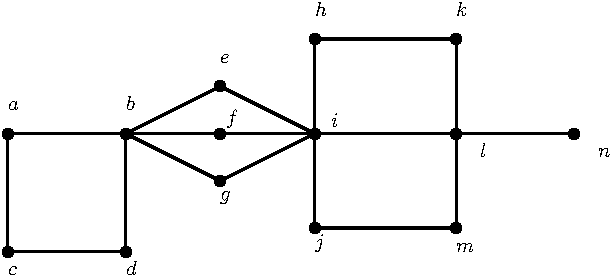
\includegraphics[scale=1]{images/graph23.pdf}
\caption{See discussion below.}
\end{figure}
In the figure above we have: $d(b, k)=4$,  $d(c,m)=6$, ecc$(a)=5$, ecc$(c)=$ecc($h)=$ecc$(m)=$ecc($n)=6$, rad$(G)=3$, center$=\{e,f,g\}$, diam$(G)=6$, periphery$=\{c,h,m,n\}.$
\begin{rem} For a cycle or a complete graph, the radius and the diameter are equal. 
\end{rem}
\begin{thm} For any connected graph $G$, rad$(G) \leq$diam$(G) \leq 2 $rad$(G)$. 
\end{thm}
\begin{proof}
Clearly rad$(G) \leq$diam$(G)$. Let $u,v \in V$ such that $d(u,v)=$diam$(G)$. Let $c$ be in the center of $G$. Then diam$(G)=d(u,v) \leq d(u,c) \leq d(c,v) \leq 2 $ecc$(c)=2$rad$(G)$. 
\end{proof}
\begin{rem} We can extend these definitions to any type of simple graph. If $u$ and $v$ are in different connected components, we set $d(u,v)= \infty$. 
\end{rem}
\newpage
\begin{thm} Every graph $G$ is the center of some graph. 
\end{thm}
\begin{proof}
We construct a new graph by adding four vertices $(w, x,y,z)$ to $G$ along with the following edges: $\{wx, yz\} \cup \{ xa, a \in V(G)\} \cup \{ yb, b \in V(G)\}.$ 
\begin{figure}[hbtp]
\centering
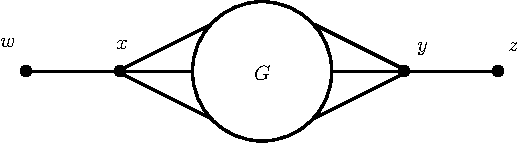
\includegraphics[scale=1]{images/graph24.pdf}
\caption{The new constructed graph.}
\end{figure}\\
Now ecc$(w)=$ecc$(z)=4$,  ecc$(y)=$ecc$(x)=3$ and for every $x \in V(G)$,  ecc$(x)=2$. Therefore $G$ is the center of this new constructed graph. 
\end{proof}
\begin{thm} \label{prevthm} Let $G=(V,E)$ be a graph of order $\geq 3$. Then $G$ is connected iff it has two distinct vertices $u$ and $v$, such that $G-u$ and $G-v$ are connected. 
\end{thm}
\begin{proof}
$(\Rightarrow)$: Let $k=diam(G)$ and let $u$ and $v$ be such that. $d(u,v)=k$. Let $P=u_0…u_k$ be a $(u,v)$-geodesic ($u_0=u, u_k=v$). Let us show that $G-u$ is connected. By definition of diameter, every $x \in V(G)$ is in P. Let $\{x,y\}$ be a pair of vertices in $G-u$. There exists a path $P’$ in $G$ joining $x$ to $y$. If $u$ is not in $P’$, then $P’$ is also a path in $G-u$ as well. If not, the predecessor of $u$ in $P’$ is a vertex $v_i \in P$ and the successor of $u \in P’$ is a vertex $v_j \in P$. We now take the part in $P’$ from $x$ to $v_i$, then the part $v_i$ to $v_j \in P$, and $v_j$ to $y$ in $P’$. Hence there exists a path from $x$ to $z$ in $G-u$ and $G-u$ is connected. We show in  exactly the same way that $G-v$ is connected.\\
$(\Leftarrow)$: Let $x,y$ be two vertices of $G$. 
\underline{case1:} $\{x,y\}\neq \{u,v\}$, for instance $u\neq x, u\neq y$. Then $x$ and $y$ are in $G-u$. As $G-u$ is connected, there is a path from $x$ to $y$ in $G-u$ and hence in $G$.\\
\underline{case2:} $\{x,y\}=\{u,v\}$. For instance $x=u, y=v$. $|G| \geq 3$. Hence there exists $w \in V(G)$, $w\neq u, w\neq v$. $G-v$ is connected, so there exists a  $(u,w)$-walk in $P’$ and similarly there exists a $(v,w)$-walk in $P"$. Then $P’ \cup P"$ is a $(u,v)$-walk in G.
\end{proof}
\begin{thm} Let $G$ be a simple graph, $|G|=n, \ |E(G)|=m$, such that $G$ has $q$ connected components. Then we have:
\begin{align*}
n-q \leq m \leq \frac{(n-q)(n-q+1)}{2}
\end{align*}
\end{thm}
\begin{proof}
We are going to show that $n-q \leq m$. It suffices to show it for $q=1$ (i.e. a connected graph): the general case follows by addition of each connected component. The property is obvious for $n=1$ and $n=2$.
\\
\\ Suppose $n \geq 3$. We show that $n- 1 \to n$. Let $G=(V,E)$ be a graph of order $n$. Let $v \in V$ be such that $G \setminus v$ is connected (such a vertex exists according to the previous theorem, i.e. Theorem \ref{prevthm}). We then have $|E(G \setminus v)| = m' \leq m-1$. 
\\\\
It follows from the induction assumption that $m' \geq (n-1)-1 $ which implies that $m \geq n-1.$ Next we show that 
\begin{align*}
m \leq \frac{(n-q)(n-q-1)}{2},
\end{align*}
with an induction on $q$. For $q=1$, the statement is obviously true. Let us thus assume $q \geq 2$. We show $q-1 \to q$. Let $G(V,E)$ be a graph with $n$ vertices, $q$ connected components and $m$ edges. Let $G_1=(V_1,E_1)$ be a connected component of $G$ of order $n_1$. The graph $G-V_1$ has $n-n_1$ vertices and $q-1$ connected components. 
\\\\
We then have:
\begin{align*}
|E(G_1)| & \leq \frac{n_1(n_1-1)}{2}, \\
|E(G_1-V_1)| & \leq \frac{((n-n_1)-(q-1))((n-n_1)-(q-1)+1)}{2}
\end{align*}
and $m=|E(G)|= |E(G_1)|+|E(G-V_1)|.$ Hence we obtain:
\begin{align*}
m & \leq \frac{n_1(n_1-1)}{2}+ \frac{(n-n_1-q+1)(n-n_1-q+2)}{2} \\
& \leq \frac{(n-q)(n-q+1)}{2}-(n_1-1)(n-q-n_1+1).
\end{align*}
But $n_1 \geq 1$ and $n \geq m + q-1$ because each connected component must have at least one vertex. 
\end{proof}
\newpage
Next we show how one can naturally associate a matrix to a graph.
\begin{defn} Let $G=(V,E)$ be a general graph and note $V(G)=\{v_1, \dots , v_n\}.$ The \textbf{adjacency matrix} of $G$ is the $n \times n$, noted $A_G=A=(a_{ij})_{1 \leq i,j \leq n}$ defined  as
\begin{align*}
a_{ij} = \begin{cases} \# \text{ edges that are incident to $v_i$ and $v_j$}, & i \neq j \\ \# \text{ of loops incident to $v_i$}, & \text{otherwise} \end{cases}
\end{align*}
\end{defn}
\begin{rem} Note that $A$ is always symmetric and that for a simple graph, the entries or either $0$ or $1$. 
\end{rem}
From now on, unless stated otherwise, we focus on simple graphs. 
\begin{exmp} \label{exmpref} \
\begin{figure}[hbtp]
\centering
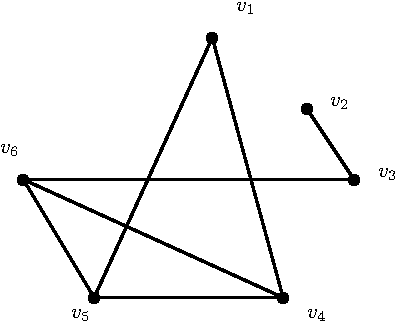
\includegraphics[scale=1]{images/graph25.pdf}
\caption{A graph $G$ on $6$ vertices with adjacency matrix $A$ given below.}
\end{figure}
\begin{align*} A=
\begin{pmatrix}
0 & 0 & 0 & 1 & 1 & 0 \\
0 & 0 & 1 & 0 & 0 & 0 \\
0 & 1 & 0 & 0 & 0 & 1 \\
1 & 0 & 0 & 0 & 1 & 1 \\
1 & 0 & 0 & 1 & 0 & 1 \\
0 & 0 & 1 & 1 & 1 & 0 
\end{pmatrix}.
\end{align*}
\end{exmp}
\begin{thm} Let $G=(V,E)$ be a (simple) graph of order $n$ and let $k \in \mathbb{N}$. Let $A$ be the adjacency matrix of $G$, corresponding to $V= \{v_1, \dots , v_n\}.$ Then the number of walks of length $k$ between $v_i$ and $v_j$ is the $(i,j)$-th entry of the matrix $A^k$. 
\end{thm}
\newpage
\begin{proof}
We note $A=(a_{ij})$ and $A^k=(a_{ij}^k)$. We prove the result with an induction on $k$. For $k=1$, the property follows from the definition of an adjacency matrix.  \\\\
$k \to k+1$. A walk of length $(k+1)$ between $v_i$ and $v_j$ is the union of a walk of length $k$ between $v_i$ and another vertex $v_h$, and an edge between $v_h$ and $v_j$. We deduce from the induction assumption that the number of walks of length $k+1$ between $v_i$ and $v_j$ is :
\begin{align*}
\sum_{h=1}^n a_{ih}^{(k)} a _{hj} = a_{ij}^{(k+1)}. 
\end{align*}
\end{proof}
\begin{exmp} In the case of Example \ref{exmpref}, we have $a_{1,6}^{(3)}=1.$
\end{exmp}
\begin{thm} Let $G$ be a simple graph on $n$ vertices, and let $A$ be its adjacency matrix. Then $G$ is connected iff $(I+A)^{n+1}$ consists of strictly positive entries.
\end{thm}
\begin{proof}
We know that if there is a walk from $v_i$ to $v_j$ in $G$, then there is a path too. The length of a path in $G$ is at most $n-1$. Therefore $G$ is connected iff for any pair of vertices $v_i$ and $v_j$ there is a positive integer $k \leq n-1$ such that $a_{ij}^{(k)} >0$. Moreover we have
\begin{align*}
(I+A)^{n+1} = \sum_{k=0}^{n-1} {n-1 \choose k } A^k,
\end{align*}
and the statement follows. 
\end{proof}
More generally let us note $S_k = I + A + \dots + A^k$. The entries of $I$ and $A$ are either $0$ or $1$. So the entries of $S_k$ are positive integers. In particular $(S_k)_{i,j} \leq ( S_{k+1})_{i,j}$.
\begin{thm} Let $G$ be a connected graph with vertices labelled $v_1,v_2, \dots , v_n$ and let $A$ be its corresponding adjacency matrix. 
\begin{enumerate}
\item If $k$ is the smallest positive integer such that the $j$-th row of $S_k$ contains no zeroes, then ecc$(v_j)=k$.
\item If $r$ is the smallest positive integer such that all entries of at least one row of $S_n$ are $>0$, then rad$(G)=r$. 
\item If $m$ is the smallest integer such that all entries of $S_n$ are positive, then diam$(G)=m$. 
\end{enumerate}
\end{thm}
\newpage
\section{Coloring}
\begin{defn} Let $G$ be a simple graph and let $k \in \mathbb{N}, k >0$. A \textbf{$k$-coloring} of the vertices of $G$ is an application $g: V(G) \to \{1, \dots ,  k \}$ such that if $\{u,v\} \in E$, then $g(u) \neq g(v)$. A graph for which a $k$-coloring exists is said to be \textbf{$k$-colorable}. Note that a graph of order $n$ is always $n$-colorable. Hence for every simple graph $G$, there exists a smallest integer $k$ such that $G$ is $k$-colorable. This number is called the \textbf{chromatic number} of $G$ and is noted $\chi(G)$. 
\end{defn}
\begin{rem} A graph $G$ is $k$-colorable iff it is $k$-partite.
\end{rem}
It is not an easy problem to find in practice the chromatic number of $G$. We now propose an algorithm,  called the \textbf{greedy algorithm}, which allows us to find a coloring for a given graph $G$. 
\\\\
\textbf{Algorithm:} The algorithm proceeds as follows: we consider an enumeration $v_1, \dots , v_n$ of the vertices of $G$. We associate the color $0$ to $v_1$. Then we associate color $1$ by going through the list $v_2, \dots , v_n$ to all vertices, which are not adjacent to a vertex which is already colored. If after this process, there are vertices which are not colored yet, we associate color $2$ to the first non colored vertex and proceed as before, until all vertices are colored. 
\begin{rem}
This algorithm provides us with a $k$-coloring with $k > \chi(G)$. But it does not necessarily give $\chi$. Let us for instance consider $P_5$ as depicted in the figure below: 
\begin{figure}[hbtp]
\centering
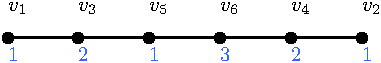
\includegraphics[scale=1]{images/graph26.pdf}
\caption{The greedy algorithm gives $h=3$ but $\chi=2$. }
\end{figure}
\end{rem}
\begin{thm} Let $G$ be a simple graph with maximal degree $\Delta(G)$ and chromatic number $\chi(G)$. Then we have:
\begin{align*}
\chi(G) \leq \Delta(G) +1. 
\end{align*}
\end{thm}
\begin{proof}
If $G$ is colored following the greedy algorithm, with $k$ colors, then the last colored vertex is adjacent to one vertex of the $k-1$ first colors, for otherwise it would have been colored with one of these colors. The degree of these vertices is $\geq k-1$. Hence $\Delta(G) \geq k-1 \geq \chi(G)-1$. 
\end{proof}
\begin{rem}
Note that the $k$-cycle $C_k$, with $k$ odd, and the complete graph $K_n$ satisfy $\chi(C_k)=\Delta(C_k)+1$ and $\chi(K_n)=\Delta(K_n)+1$. In fact,  in can be shown that these are the only graphs with this property. For all other types of graphs, we have $\chi(G) \leq \Delta(G)$. 
\end{rem}
\section{Trees}
\begin{defn} A \textbf{forest} is a graph without cycles (or acyclic). A \textbf{tree} is a connected and acyclic graph. Note that the connected components of a forest are trees. In general, in a graph, a vertex of degree $1$ is called a\textbf{ leaf}.
\end{defn}
\begin{exmp} \
\begin{figure}[hbtp]
\centering
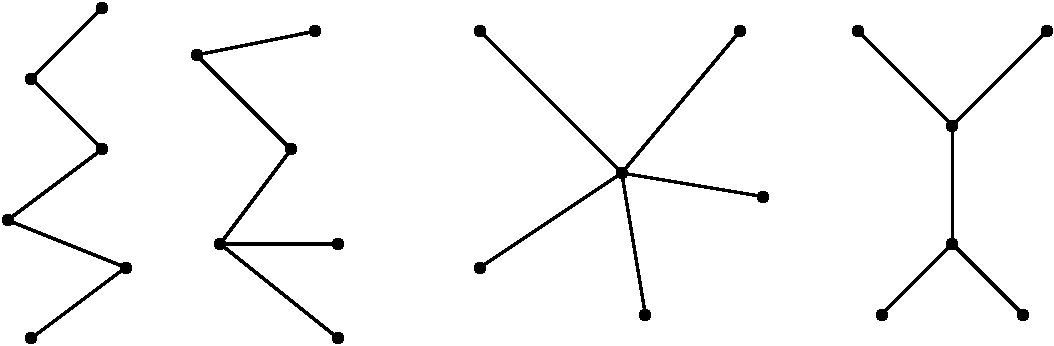
\includegraphics[scale=.7]{images/graph27.pdf}
\caption{Trees on six vertices.}
\end{figure}
\end{exmp}
\begin{thm} Let $G=(V,E)$ be a forest, such that $E \neq \emptyset$. Then $G$ has at least two leaves. 
\end{thm}
\begin{proof}
Let $C=(v_0,e_1, \dots , e_k,v_k)$ be a path of maximal length in $G$. Since $E \neq \emptyset$, $k \geq 1$. Assume that $d(v_k) >1$. Since $G$ is acyclic, there is a vertex $v \notin \{ v_0, \dots , v_{k-1}\}$ which is adjacent to $v_k$. But this contradicts the maximality of $C$. Hence $d(v_k)=1$. Similarly we have $d(v_0)=1$. 
\end{proof}
\begin{cor} A tree $G=(V,E)$, with $|V| \geq 2$, has at least two leaves.
\end{cor}
\begin{lem} A tree of order $\geq 2$ is bipartite, and also $2$-colorable. 
\end{lem}
\begin{proof}
Follows from the fact that a graph without odd cycles is bipartite. 
\end{proof}
\newpage
Next we state in a single theorem a lost of fundamental properties of trees.
\begin{thm} \label{chartreethm} Let $G=(V,E)$ be a graph with $n$ vertices and $m$ edges. The following properties are equivalent:
\begin{enumerate}
\item The graph $G$ is a tree.
\item The graph $G$ is connected and $m=n-1$.
\item The graph $G$ is acyclic and $m=n-1$.
\item For every pair of vertices $\{x,y\},$ there exists a unique $(x,y)$-path.
\item The graph $G$ is connected and for every $e \in E$, $G-e$ is not connected.
\item The graph $G$ is acyclic, and for all pairs of vertices $\{x,y\},$ which are non adjacent, $(V,E \cup \{x,y\})$ has a cycle. 
\end{enumerate}
\end{thm}
\begin{proof}
i) $\implies$ ii) and iii). We prove with an induction on $m=n-1$. For $n=1$, $G$ is an isolated vertex and the statement is obvious. 
\\
$n-1 \implies n$. Let $G$ be a tree on $n$-vertices. $G$ has at least two leaves. Let $v_0$ be a leaf. Then $G-v_0$ has $n-1$ vertices and is a tree. It follows from the induction assumption that it has $n-2$ edges. So $G$ has $n-1$ vertices.\\
\\
ii) $\implies$ i) We shall again proceed with an induction. We first note that for $n \geq 2$. such a graph has at least one leaf. Such a graph does not have a vertex of degree $0$ because it is connected, on the other hand if all degrees are $\geq 2$, then $\sum d(v) \geq 2n$, but we know that $\sum d(v) = 2|E|=2n-2$ and this is a contradiction. 
\\\\
For $n=1$, the graph is just a single vertex and is thus a tree. \\
$n \geq 2, n-1 \to n$. Let $v_0$ be a leaf of $G$. $G-v_0$ is connected and has $n-2$ edges. So by the induction assumption, it is a tree. Consequently $G$ is a tree. \\
\\
i) $\implies$ iv) Let $G$ be a tree and $\{x,v\} \subset V$. $G$ is connected, so there is a $(x,y)$-path. Let us assume that there exists two such $(x,y)$-paths, say $C_1$ and $C_2$ such that $C_1 \neq C_2$. Then there exists at least one edge in $C_1$ and not in $C_2$. For instance $e=\{z,t\}.$ The subgraph of $G$, union of $C_1$ and $C_2$ minus $e$ would be connected and would contain a $(z,t)$-path. Adding $e$ to this path we would obtain a cycle. Which is a contradiction.
\\\\
iv) $\implies$ i) It follows from iv) that $G$ is connected. If $G$ contains a cycle this cycle would contain at least two different vertices and have two distinct $(x,y)$-paths. 
\newpage
iv) $\implies$ v) Let $E$ be a vertex, $e=\{x,y\}.$ Then $(x,e,y)$ is a $(x,y)$-path, and by  assumption, it is the unique $(x,y)$-path. The graph $G-e$ does not have $(x,y)$-paths and hence is not connected. 
\\\\
iv) $\implies$ vi) We have already seen that  iv $\implies$ $G$ is acyclic. Let $x,y$ bet wo non adjacent vertices of $G$. There exists a unique $(x,y)$-path. If we add $\{x,y\}$, then we have a (unique) cycle. \\
\\
vi) $\implies$ i) We only need to prove that vi) implies that $G$ is connected. Let $x,y \in V(G)$. If $x$ and $y$ are adjacent,  then there is a $(x ,y)$-path. If $x$ and $y$ are not adjacent, then adding $\{x,y\}$ creates a cycle and we then have a $(x, y)$-path in $G$. 
\end{proof}
Recall that a spanning subgraph of a graph $G$ is a subgraph of $G$ with vertex set $V(G)$. 
\begin{defn} A \textbf{spanning tree} of a graph $G$ is a spanning subgraph of $G$ which is also a tree. 
\end{defn}
\begin{thm} A graph $G$ is connected iff it has a spanning tree.
\end{thm}
\begin{proof}
Let $G'$ be a spanning subgraph of $G$, which is connected and minimal in the sense that if $e' \in E(G')$,  then $G'-e'$ is not connected. It follows from Theorem \ref{chartreethm} that $G'$ is a tree. The converse is obvious (by truncation). 
\end{proof}
\begin{cor} Let $F$ be a forest on $n$ vertices with $k$ connected components. Then $F$ has $n-k$ edges. 
\end{cor}
\begin{proof}
This follows immediately by using a simply counting argument on the number of vertices. 
\end{proof}
\newpage
Now we would like to ask how many trees there are on $n$ vertices. We denote $[n]:= \{1,2, \dots ,  n \}$ as the vertex set. 
\begin{thm}[Cayley's formula] For $n \geq 1$, the number of all trees with vertex set $[n]$ is denoted as $A_n$ and it holds that 
\begin{align*}
A_n = n^{n-2}.
\end{align*}
\end{thm}
This is a fundamental result of graph theory and there exists many proofs for this result. We shall give three of them here.
\begin{proof}[Proof 1] Take all $A_n$ trees on $[n]$ and in each of them,  choose two vertices, which are also not have to be different, and call one of them Start and the other one End. Do this in all possibly $n^2$-ways for each tree. Call the $n^2A_n$ objects obtained this way \textbf{doubly rooted trees}.
\\\\
We are going to show that the number of doubly rooted trees on $[n]$ is $n^n$ by constructing a bijection from the set of all functions from $[n]$ to $[n]$ to that of doubly rooted trees on $[n]$. Let $f: [n] \to [n]$ be a function. Let $C \subset [n]$ be the subset of elements $x \in [n]$ which are part of a cycle under the action of $f$, that is,  there is a positive $i$ such that $f^i(x)=x$. Let $C=\{c_1 < c_2< \dots < c_k \}.$ Now let $d_i = f(c_i)$ and write the integers $d_1, d_2, \dots , d_k$ in order to the nodes of a tree of a tree consisting of one of $k$ vertices. Also we mark $d_1$ with Start and $d_k$ by End. 
\\\\
Finally,  if $j \in [n]$, but $j \notin C$, then join the vertex $j$ to the vertex $f(j)$ by an edge. This way we always get a tree. Indeed, we get a connected graph as the Start-End tree is connected to all vertices and we get a cycle free graph as the only cycles created by $f$  involved elements from G are the vertices $F$ in $G$, and $C$ corresponds to a single line. The tree is doubly rooted. \\
\\
To see that this is a bijection,  take a doubly rooted tree on $[n]$. For vertices $j$ not in the Start-End line,  define $f(j)$ to be the first neighbor of $j$ in the unique path from $j$ to the Start-End line. For the vertices on the $S-E$ line,  define $f$ so that the image of the $i$-th smallest of them is the one that is in the $i$-th position from Start. 
\end{proof}
\newpage
In order to get a better understanding of the previous proof, we will work through an explicit example below. 
\begin{exmp} Let $n=8$ and $f:[8] \to [8]$ be defined by: 
\begin{align*}
f(1)=3, \ f(2)=4, \ f(3)=1, \ f(4)=5, \ f(5)=5, \ f(6)=7, \ f(7)=8, \ f(8)=6.
\end{align*}
$C= \{1,3,5,6,7,8\}.$ So the function $f$ creates the cycles $(1 \ 3),$ $(5)$ and $(6 \ 7 \ 8)$. So we can graphically represent the action of $f$ as:
\begin{figure}[hbtp]
\centering
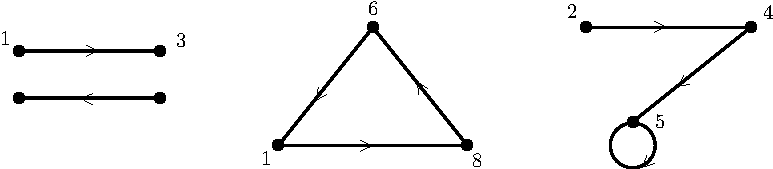
\includegraphics[scale=1]{images/graph28.pdf}
\caption{Graphical representation of the action of $f$.}
\end{figure}
\\
We thus have $d_1=3, d_2=1,  d_3=5, d_4=7, d_5=8, d_6=6$. Therefore one Start-End line will contain the integers $3,1,5,7,8,6$. \\\\
As $f(2)=4$ and $f(4)=5$, we connect the vertex $2$ to $4$ and the vertex $4$ to $5$. And we obtain the doubly rooted tree depicted in the figure below.
\begin{figure}[hbtp]
\centering
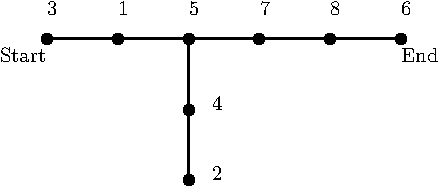
\includegraphics[scale=1]{images/graph29.pdf}
\caption{The doubly rooted tree obtained by our process.}
\end{figure}
\end{exmp}
\newpage 
\textbf{Exercise:}
\begin{figure}[hbtp]
\centering
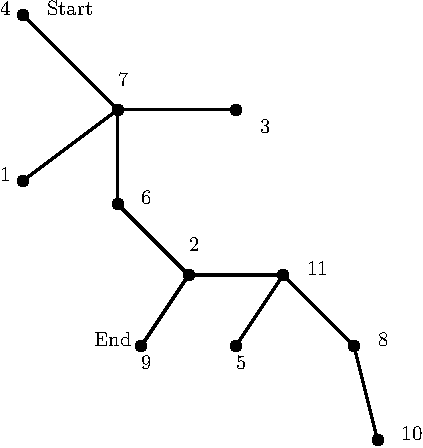
\includegraphics[scale=1]{images/graph30.pdf}
\caption{What is the function $f$ associated with the above tree?}
\end{figure}
\\
The answer is given by: $f(1)=7, f(2)=4, f(3)=7, f(4)=7, f(5)=11, f(6)=6, f(7)=2, f(8)=11, f(9)=9, f(10)=8, f(11)=2$. 
\begin{defn} To the analogy of doubly rooted trees, we can define \textbf{rooted trees}, which are trees with one vertex called the root. SO the number of rooted trees on $[n]$ is $n^{n+1}$. A \textbf{rooted forest} is a forest in which each component is a rooted tree. 
\end{defn}
\begin{cor} For all positive integers $n$, the number of rooted forests on $[n]$ is $(n+1)^{n+1}$. 
\end{cor}
\begin{proof}
Take a rooted forest on $[n]$ and join all roots to the next vertex $n+1$. This transforms the original rooted forest to an unrooted tree on $[n+1]$. This map is a bijection: given a tree on $[n+1]$, we can simply mark all neighbours of $n+1$ as roots, then delete all edges adjacent to $n+1$, to get the original rooted forest back. So the set of all rooted forests on $[n]$ is in bijection with that of all trees on $[n+1]$ and therefore there are $(n+1)^{n+1}$ of them. 
\end{proof}
\newpage
Now we provide another proof of Cayley's Theorem,  due to Pitman as a problem with solution. 
\begin{proof}[Problem: Pitman's proof of Cayley's theorem] Let $F$ be a rooted forest on $n$ vertices and view $F$ as a directed graph, in which all edges are directed from the roots. If $F'$ is another rooted forest,  then we say that $F$ contains $F'$ if $F$ contains $F'$ as a directed graph. Clearly, in that case $F$ has less components than $F'$. We say that $F_1, F_2, \dots ,  F_k$ is a \textbf{refining sequence} if for all $i \in [k]$,  $F_i$ is a rooted forest on $[n]$ having $i$ components, and $F_i$ contains $F_{i+1}.$ Now fix $F_k$. 
\begin{enumerate}[label=(\alph*)]
\item Find the number $N^*(F_k)$ of refining sequences ending in $F_k$.
\item Find the number $N(F_k)$ of rooted trees containing $F_k$.
\item Deduce Cayley's formula. 

\end{enumerate}
We now provide detailed solutions to the above questions to conclude the proof:
\begin{enumerate}[label=(\alph*)]
\item Let us build a refining sequence starting from $F_k$. First we need to choose $F_{k-1}$ by adding an edge $e$ to $F_k$. The starting vertex of $e$ can be  any of the $n$ vertices, but the ending vertex of $e$,  however must be the root of one of the components of $F_k$ not containing $e$. Therefore we have $n(k+1)$ choices for $e,$ and thus we have ```chains for $F_{k-+}$. Repeating the argument, we have $n(k-2)$ choices for $F_{k-2}$ (for each choice of $F_{k-1})$,  and so on. Therefore,  repeating the argument $k-1$ times,  we get 
\begin{align*}
N^*(F_k)=n^{k-1}(k-1)!
\end{align*}
\item If $F_1$ is a rooted tree containing $F_k$, then $F_1$ has $k-1$ more edges than $F_k$. We can remove those $(k-1)$ edges in $(k-1)!$ different ways, then obtaining 
\begin{align*}
N^*(F_k)=(k-1)! N(F_k).
\end{align*}
It follows from the above that $N(F_k)=n^{k-1}.$ 
\item Choose $k=n$. Then $F_k$ is made of rooted vertices and all rooted trees contain $F_n$. Then $N(F_n)=n^{n-1}$ is the number of all rooted trees on $[n]$. The number of unrooted trees on $[n]$ is therefore $n^{n-2}.$ 
\end{enumerate}
\end{proof}
\newpage
\textbf{Exercise:} Find a formula for the number of rooted forests on $[n]$ having $k$ components.
\begin{proof}
We have just shown that $N^*(F_n)=n^{n-1}(n-1)!$. Now let $N^{**}(F_n)$ be the number of the refining sequences $F_1, \dots , F_n$ where the $k$-th term is $F_k$. There are $N^*(F_k)$ choices for the sequence $F_1, F_2, \dots , F_k$, then there are $(n-k)!$ ways of removing the $(n-k)$ remaining edges. This shows that
\begin{align*}
N^{**}(F_k)=N^*(F_k)(n-k)!=n^{k-1}(k-1!(n-k)!
\end{align*}
This number does not depend on the choice of $F_k$ On the other hand,  each refining sequence $F_1,  F_2, \dots , F_k$ contains exactly all rooted forests of $k$ components. Therefore the number of rooted forests on $[n]$ with $k$ components is the number of all refining sequences divided by the number of refining sequences in which a sequence $F_k$ occurs. 
\begin{align*}
\frac{n^{n-1}(n-1)!	}{n^n(k-1)!(n-k)!} = {n \choose k} kn^{n-k-1}. 
\end{align*}
\end{proof}
\newpage
\textbf{Prüfer's method:} Given a tree $T$ with vertices labelled $1$ to $n$.
\begin{enumerate}
\item Let $i=0$, and $T_0=T$.
\item Find the lead on $T_i$ with the smallest label and it $v$.
\item Record in the sequence the label of $v$'s neighbor.
\item Remove $v$ from $T_i$ to crate a new `` $T_{i+1}.$
\item If $T_{i+1}=K_2$, then stop. Otherwise increment $i$ by 1 and go to step 2. 
\end{enumerate} 
\
\begin{figure}[hbtp]
\centering
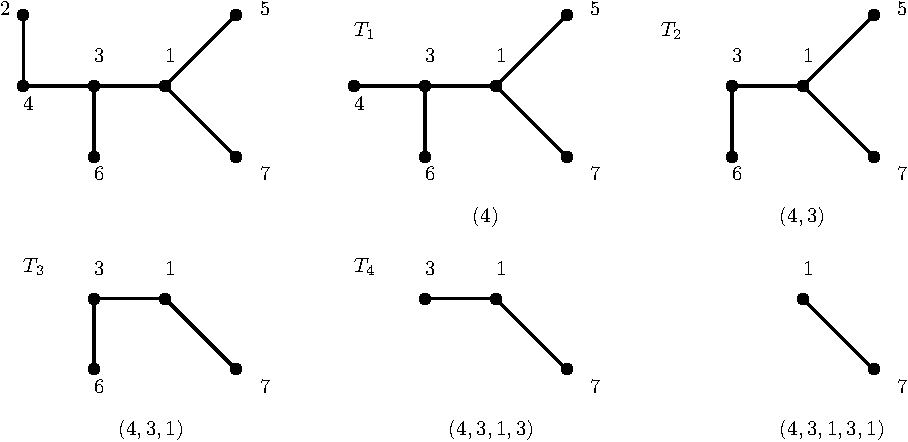
\includegraphics[scale=.8]{images/graph31.pdf}
\caption{A worked example of Prüfer's method.}
\end{figure}
\\
It can be shown that each vertex $v$ appears in the sequence exactly $d(v)-1$ times. Conversely one can associate a tree to such a sequence.  \\
Given a sequence $\delta=a_1,a_2, \dots ,  a_k$ of entries from $\{1, \dots , k-1\}$.
\begin{enumerate}
\item Draw $k+1$ vertices, label them $v_1, \dots ,  v_{k+1}$. Let $S=\{1, \dots , k+1\}. $
\item Let $i=0$, $\delta_0=\delta$, $S_0=S$.
\item Let $j$ be the smallest number in $S_i$ that does not appear in $\delta_i$.
\item Place an edge between vertex $v_j$ and the vertex whose subscript appears first in $v_i$.
\item Remove the first number in $\delta_i$ to create a new sequence $\delta_{i+1}$. Remove $j$ from $S_i$ to create a new set $S_{i+1}$
\item If $\delta_{i+1}= \emptyset$, place an edge between the two vertices whose subscripts are in $S_{i+1}$ and stop. Otherwise increment $i$ by 1 and return to step 3.
\end{enumerate}
\newpage
\begin{figure}[hbtp]
\centering
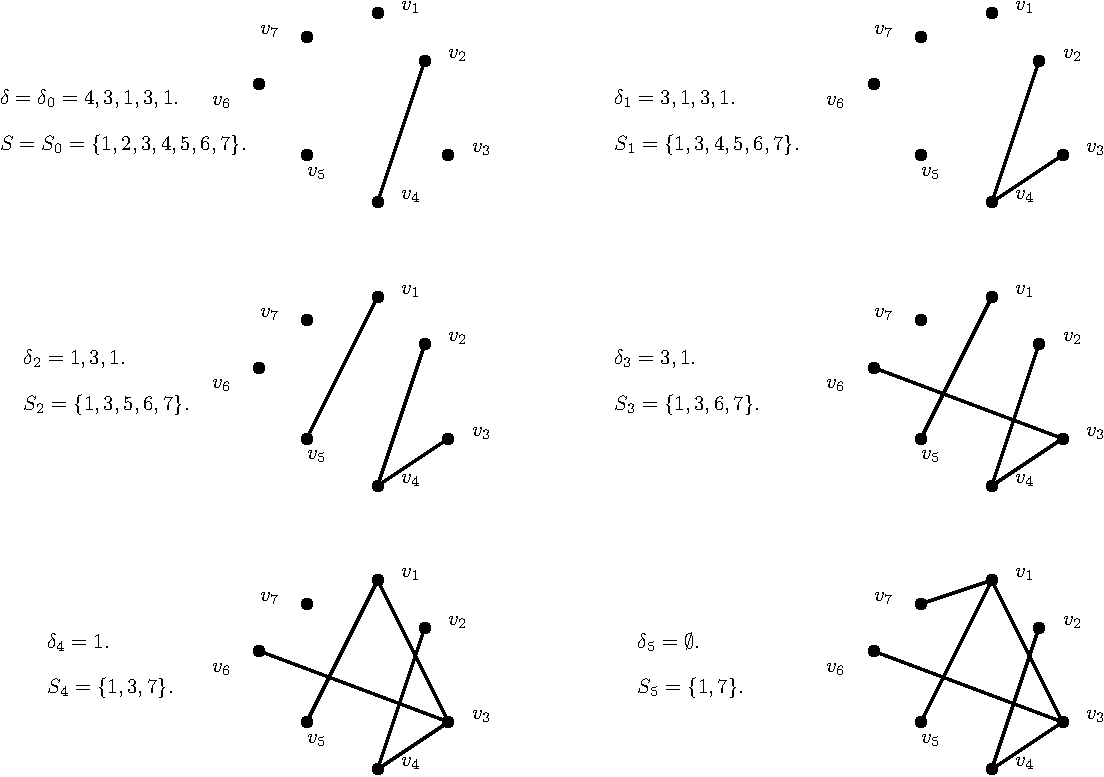
\includegraphics[scale=.71]{images/graph32.pdf}
\caption{The previous algorithm explained.}
\end{figure}
So we need to check that the Prüfer method provides us with a bijection. We take $\delta=(a_1,a_2,\dots a_{n-2})$ and we show that there exists a unique tree $T$ on $[n]$ whose Prüfer case is $\delta$. Note that the elements of $[n]$ that are not in $\delta$ must precisely be the \\\\
However in this case the degree of $j$ in the final 2-element tree is one, while its degree in the original tree was at least 2, as j was not a leaf. So again at some point a vertex was cut off from $j$, putting $j$ into $\delta$. 
So $\delta$ tells us what the leaves of the original tree were; denote them by $b_1, \dots b_n$ in increasing order. We know that first we have to cut off the leaf with the smallest label. Therefore we are reconstructing the line by joining $b_1$ to $a_1$, as $a_1$ is by definition the single neighbor of the smallest leaf. How do we know whether $a_1$ became a leaf after the first step? Iff it does not occur in delta any additional times , as in this case nothing else can be cut off from it.\\
So if $a_1$ does not occur in $S$ after the first position, then in the second step we join $min(a_1,b_2)$ to $a_2$ by an edge. Otherwise we simply join $b_2$ to $a_2$ by an edge. In general, at the $i^{th}$ step, we have to find the minimal element $b_j$ that has not been attached to any edge and the minimal element $a_k$ that has not been added to an edge yet, and does not occur in S anywhere after position $a_{i+1}$. Then we join $min(a_k,b_j)$ to $a_i$ by an edge.
\newpage
Any connected graph $G$ has at least one spanning tree. In general, a connected graph will have many spanning trees. For instance $K_n$ has $n^{n-2}$ spanning trees. 
\begin{defn} Let $G$ be a connected simple graph. Let $w: E(G) \to \mathbb{R}_+$ be a function. The function $w$ is usually called the \textbf{weight function} and $w(e)$ is called the \textbf{weight} of $e$, while for a tree $T$, $\sum_{e \in T} w(e)$ is called the weight of $T$. 
\end{defn}
\textbf{Problem:} Find the spanning tree $T$ of $G$ so that $\sum_{e \in T} w(e)$ is minimal.
\\\\
We cannot attack this problem by enumerating all possible spanning trees and compute their respective weight. For instance take $n=20$, $G=K_n$. Then we would have to compute the total weight of $20^{18} > 2.5 \times 10^{23}$ spanning trees. If one computer would could handle $10^9$ trees per second,  then it would still take $2.5 \times 10^{14}$ seconds, i.e. more than $91$ years!\\
\\
So instead, we try a smart algorithm. Take the edge with the smallest weight (or one of them if there are several), and put it in $T$. Second, take the edge that has the smallest weight among them not in $T$, and add it to $T$. In the third step and all subsequent steps,  we have to be careful. We want to make sure that by adding an edge, we will not create a cycle. 
\\\\
In general in the $i$-th step of the algorithm, we look for the edge $e_i$ that has the following properties:
\begin{enumerate}
\item the edge $e_i$ is not yet in $T$.
\item if we add $e_i$ to $T$, the obtained graph does not contain a cycle
\item the weight of $e_i$ is minimal among all edges that have properties 1), and 2).
\end{enumerate}
When we found the edge $e_i$, we add it to $T$. It is clear that we can continue this procedure until $T$ has $n-1$ edges. This algorithm is called \textbf{Kruksal's algorithm} Will it give us the minimum weight spanning tree?
\begin{lem} Let $F$ and $F'$ be two forests on the same vertex set, and let $F$ have less edges than $F'$. Then $F'$ has an edge $e$ that can be added to $F$ so that $F' \cup e$ is still a forest. 
\end{lem}
\begin{proof}
Assume that there is no such edge $e \in F'$. Then adding any edge of $F'$ to $F$ would create a cycle in $F$. So all edges of $F'$ are between two vertices of the same connected component of $F$. Therefore $F'$ has at least as many components as $F$. This is a contradiction to the assumption that $F'$ has more edges than $F$. 
\end{proof}
\begin{thm} Kruksal's algorithm always finds the minimum weight spanning tree. 
\end{thm}
\begin{proof}
Assume that Kruksal's algorithm produces a spanning tree $T$ while $G$ has a spanning tree $H$ whose total weight is less than $T$. Let $h_1, \dots h_{n-1}$ be the edges of $H$ so that $w(h_1) \leq w(h_2) \leq \dots \leq w(h_{n-1})$. Similarly let $t_1, \dots , t_{n-1}$ be the edges of $T$ such that $w(t_1) \leq w(t_2) \leq \dots \leq w(t_{n-1})$. Let $i$ be the smallest integer such that 
\begin{align*}
\sum_{j=1}^{i} w(h_j) < \sum_{j=1}^{i} w(t_j). 
\end{align*}
Such an $i$ exists by assumption on $H$. It is also clear that $i>1$,  because $w(t_1)$ is minimal. Since 
\begin{align*}
\sum_{j=1}^i w(h_j) < \sum_{j=1}^i w(t_j), \text{ and } \sum_{j=1}^{i-1} w(h_j) \geq \sum_{j=1}^{i-1} w(t_j),
\end{align*}
we must have $w(h_i) < w(t_i)$. Let $T_{i-1}$ be the forest the Kruksal's algorithm produced in $i-1$ steps, and let $H_i$ be the forest formed by the edges $h_1, \dots , h_i$. We apply the previous lemma to $T_{i-1}$ and $H_i$ we see that is an edge $h_j$ with $j \leq i$ that can be added to $T_{i-1}$ without forming a cycle. However $h_j \leq h_i < t_i$. So at step $i$, the Kruksal’s algorithm could not add  $t_i$ to $T_{i-1}$ as $t_i$ did not have minimal weight among the edges that could be added to $T_{i-1}$ without forming a cycle. This is a contradiction. 
\end{proof}
\newpage
\begin{exmp}   \
\begin{figure}[hbtp]
\centering
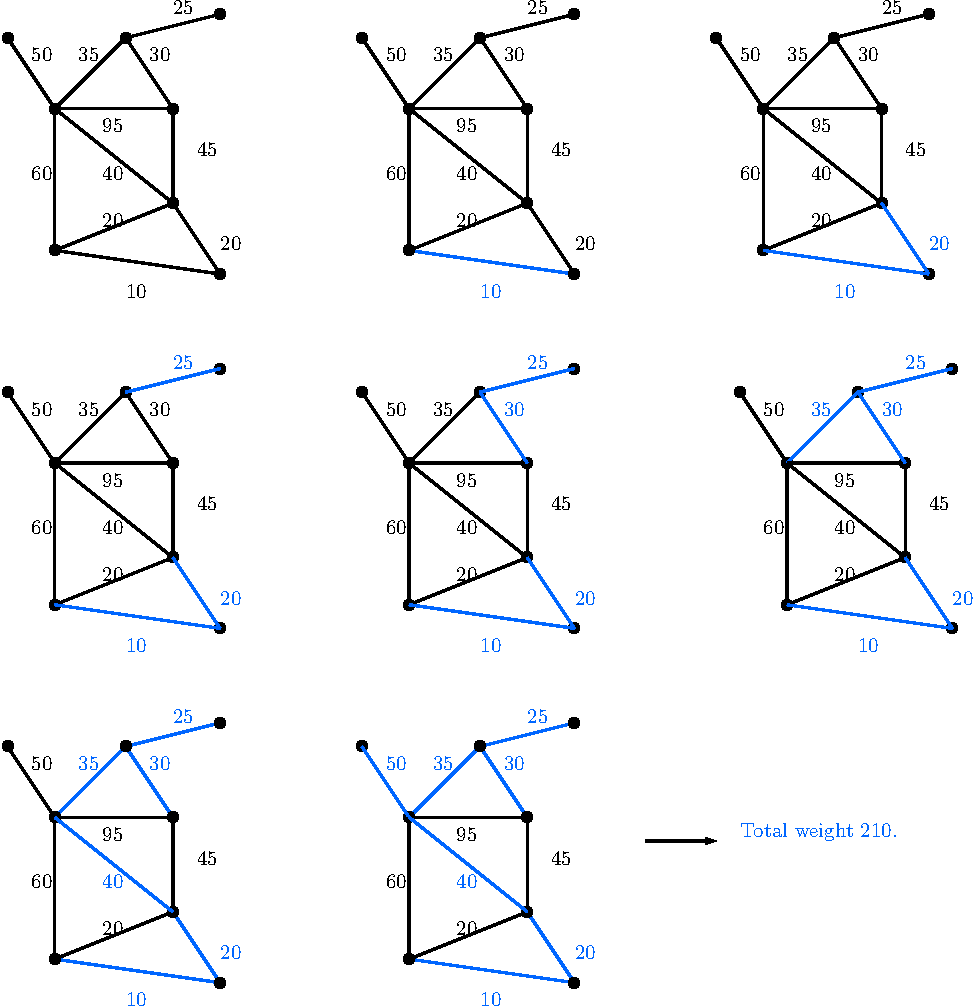
\includegraphics[scale=.85]{images/graph33.pdf}
\caption{A worked example of Kruksal's algorithm.}
\end{figure}

\end{exmp}
\newpage
\begin{thm}[Matrix Tree Theorem] Let $G$ be a connected simple graph with vertices $\{c_1, \dots ,  v_n\}$. Define $D= \text{diag}(d(v_i))_{1 \leq i \leq n}$. and let $A$ be the adjacency matrix of $G$. Then the number of spanning trees of $G$ is equal to the value of any cofactor of the matrix $D-A$. 
\end{thm}
\begin{rem} Recall that if $M=(m_{ij})_{1 \leq i,j \leq n }$ is a matrix, then the $(i,j)$ cofactor of $M$ is defined as $(-1)^{i+j} \det (M(i,j))$ where $M(i,j)$ is the matrix obtained from $M$ by deleting its $i$-th row and its $j$-th column.  
\end{rem}
\begin{exmp} \

\begin{figure}[hbtp]
\centering
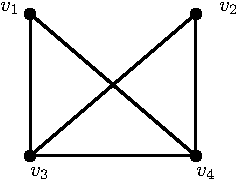
\includegraphics[scale=1]{images/graph34.pdf}
\caption{A graph on $4$ vertices to motivate the matrix tree theorem.}
\end{figure}
With the graph as depicted above we have:
\begin{align*}
A = \begin{pmatrix}
0 & 0 & 1 & 1 \\
0 & 0 & 1 & 1 \\
1 & 1 & 0 & 1 \\
1 & 1 & 1 & 0 
\end{pmatrix}, \ 
D= \text{diag}(2,2,3,3), \
D-A = \begin{pmatrix}
2 & 0 & -1 & -1 \\
0 & 2 & -1 & -1 \\
-1 & -1 & 3 & -1 \\
-1 & -1 & -1 & 3
\end{pmatrix}. 
\end{align*}
The cofactor of $(1,1)$ is given by 
\begin{align*}
\det \begin{pmatrix}
2 & -1 & -1 \\
-1 & 3 & -1 \\
-1 & -1 % 3
\end{pmatrix} = 8.
\end{align*}
\end{exmp}
\textbf{Exercise:} Use the matrix tree theorem to prove that the number of trees on $n$ vertices is $n^{n-2}$. 
\begin{proof}
\begin{align*}
\det \begin{pmatrix}
n-1 & -1 & \dots & -1 \\
-1 & \ddots & -1 &  \vdots \\
\vdots & & \ddots  & -1 \\
-1 & \dots & -1 & n-1
\end{pmatrix} = n^{n-2}.
\end{align*}
\end{proof}
\textbf{Exercise:} Find the number of spanning trees of $K_{m,n}.$ \\
\textbf{Answer:} $m^{(n-1)} \cdot n^{(m-1)}$
\newpage
\section{Eulerian trails and Hamiltonian cycles}
\begin{defn} If a trail in a graph $G$ includes every edge of $G$, then that trail is said to be an \textbf{Eulerian trial}. Similarly an \textbf{Eulerian circuit} in a graph is a circuit that includes every edge of the graph. A graph that contains an Eulerian circuit is called an \textbf{Eulerian graph}.
\end{defn}
\begin{exmp} The cycles $C_n$ are Eulerian graphs. But of course the paths $P_n$ are not.
\end{exmp}
\begin{thm} \label{thm420} For a connected graph $G$, the following statements are equivalent:
\begin{enumerate}
\item $G$ is Eulerian.
\item Every vertex of $G$ has even degree.
\item The edges of $G$ can be partitioned into edge disjoint cycles.
\end{enumerate}
\end{thm}
\begin{proof}
$1 \implies 2$. Let $C$ be an Eulerian circuit. Let $v$ be an arbitrary vertex of $G$. Every time the circuit enters $v$ or an edge, it must leave on a different edge, there must then be an even number of edges incident with $v$ and hence $d(v)$ is even.
\\
\\
$2 \implies 1$. Take any vertex $v$, and start walking along an edge $e_1$ to the other endpoint $a_1$ of that edge, then walk along a new edge $e_2$ that starts in $a_1$. Continue this way using new  edges at each step, until a closed trail $C_1$ is found. As $G$ is finite, such a trail will always be formed. The first closed trail will be found when we first visit a vertex already visited.
\\\\
If $C_1 =G$ we are done. If not, since $G$ is connected, we can have a vertex $v$ in $C_1$ so that $C_1$ does n ot contain all edges adjoint to $v$. Let us now unite all edges of $C_1$ from $G$. We get a graph in which again all vertices have even degree. Starting at $v$, let us take another closed trail $C_2$ in the remaining graph. We can then unite $C_1$ and $C_2$ into one closed trail in $G$. Indeed if we start walking b< $w_1$, we can stop at $v$, walk through $C_2$ and complete our trail by using the remaining part of $C_1$. If the new trail $C_1 \cup C_2$ contains all edges of $G$, we are done. If not, then let us emit $C_1 \cup C_2$ from $G$ and find a new closed trail $C_3$ in the remaining graph. As $G$ has a finite number of edges, the procedure has to stop after a finite number of steps. Therefore after a finite number of steps $C_1 \cup C_2 \cup \dots \cup C_k$ will be a closed trail containing all edges of $G$. 
\end{proof}
\newpage
\begin{figure}[hbtp]
\centering
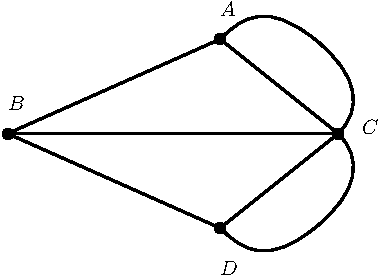
\includegraphics[scale=1]{images/graph35.pdf}
\caption{The graphs of the Königsberg bridges.}
\end{figure}
We cannot walk through all bridges of Königsberg so that we start and end where we started, and use each bridge exactly once. 
\begin{cor} Let $G$ be a connected graph. Then $G$ has an Eulerian trail starting at vertex $u$ and ending at a different vertex $v$ iff $u$ and $v$ have odd degree, and all other vertices of $G$ have even degree. 
\end{cor}
\begin{proof}
Add a new edge joining $u$ and $v$, and call the new graph obtained $H$. Then $H$ has a Eulerian circuit iff $G$ has an Eulerian trail from $u$ to $v$. 
\end{proof}
\begin{rem} The proof we have for Theorem \ref{thm420} allows us to find an Eulerian circuit. 
\begin{figure}[hbtp]
\centering
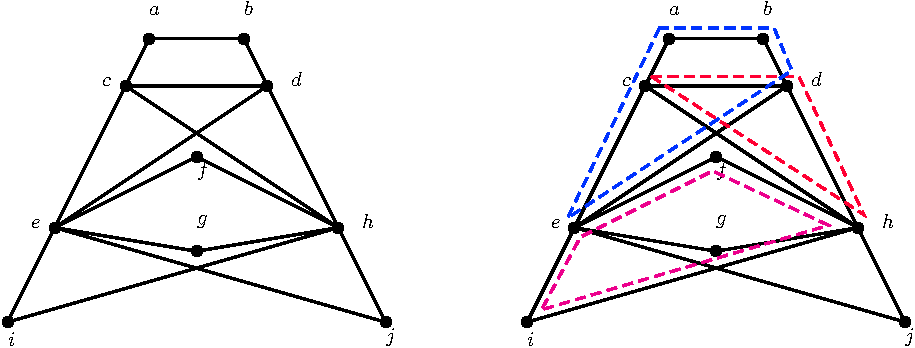
\includegraphics[scale=.9]{images/graph36.pdf}
\caption{Shows how to find an Eulerian circuit.}
\end{figure}
\end{rem}
\newpage
\begin{defn} Let $G$ be a graph. If a path $P$ spans the vertices of $G$, i.e. $V(P)=V(G)$, then $P$ is said to be a \textbf{Hamiltonian path}. Any graph $G$ containing a Hamiltonian path is called \textbf{traceable}. If a cycle spans the vertices of a graph $G$, such a cycle is called a \textbf{Hamiltonian cycle} and any graph containing a Hamiltonian cycle is called a \textbf{Hamiltonian graph}.  
\end{defn}
\begin{rem} Hamiltonian graphs are clearly traceable, but the converse is not always true. 
\end{rem}
\begin{thm} Let $G$ be a graph of order $n \geq 3$. If $\delta(G) \geq n/2$, then $G$ is Hamiltonian. 
\end{thm}
\begin{proof}
Let us assume that $G$ does not contain a Hamiltonian cycle. Let us add to $G$ a new edge as long as we can without creating a Hamiltonian cycle. When we stop we have a graph $G'$ in which all vertices have degree $\geq n/2$, there is no Hamiltonian cycle, but adding one new edge would create a Hamiltonian cycle. 
\\\\
Let $x$ and $y$ be two vertices in $G’$ that are not connected by an edge. If adding the edge $xy$ would create a Hamiltonian cycle, it follows that $G’$ has a Hamiltonian path $P$ that starts at $x$ and ends at $y$. Let $x=z_1,z_2, \dots , z_n-1, z_n=y$ be the vertices of this path. Therefore the pigeonhole principle implies that there must be an index $i$ so that $2\leq i \leq n$, whole $xz_i$ is an edge and whole $z_i-1y$ is also an edge. Indeed, if this was not the case, then for any neighbor $z_{i-1}$ of $y$ on $P$, $z_i$ is not a neighbor of $x$.
\end{proof}
We have the following more general theorem:
\begin{thm} Let $G$ be a simple graph of order $\geq 3$. Assume that for all $(u,v) \in V(G) \times V(G)$ such that $\{u, v\} \in E(G)$ we have $d(u) + d(v) \geq n.$ Then $G$ is Hamiltonian. 
\end{thm}
\begin{proof}
We start as in the previous proof with a maximal Hamiltonian graph and prove that in this case there exists $u,v$ non adjacent such that $d(u) \leq d(v) \leq n-1.$ There exists a no adjacent pair of vertices $u,v,$ such that $G+\{u,v\}$ is Hamiltonian. Let $C$ be a Hamiltonian cycle of $G+\{u,v\}$. $C-\{u,v\}$ is a Hamiltonian path in $G$. Let us note $(v_1, \dots ,  v_n)$ for this path, with $v_1=u$, $v_n=v$. Let $i \in \{1, \dots ,  n-1\}$ be such that $\{v_i , v_{i+1}\}$ and $\{v_n, v_i\} \in E(G)$. Then this would be a Hamiltonian cycle, which is not possible. 
\newpage
Let us thus set 
\begin{align*}
I&= \{i \in \{1, \dots ,  m-1\} \mid \{v_1v_{i-1} \} \in E(G) \}. \\
J&= \{i \in \{1, \dots , n-1\} \mid \{v_n , v_i\} \in E(G) \}. 
\end{align*} 
It it follows from the previous remark that $I \cap J = \emptyset$. Therefore $|I|+|J| = | I \cup J| \leq n-1$. We note that $|I|=d(u)$ and $|J|=d(v)$, thus $d(u) \leq d(v) \leq n-1$. 
\end{proof}
\begin{rem}Note that the above theorem does not admit a converse. For instance $C_n$ for $n \geq 5$ is Hamiltonian but $d(u)= d(v)=4 < n =5$.
\end{rem}
\begin{prop} Let $G$ be a simple graph of order $n$ with two non adjacent vertices, such that $d(u)=d(v) \geq n$. Then $G+\{u,v\}$ is Hamiltonian iff $G$ is Hamiltonian. 
\end{prop}
\begin{proof}
If $G$ is Hamiltonian, obviously $G+\{u,v\}$ is also Hamiltonian. Let us assume that $G$ is not Hamiltonian. and that there exists two non adjacent vertices $u,v$ such that $G+\{u,v\}$ is Hamiltonian. But then every Hamiltonian cycle would include $\{u,v\}$ and then $G$ would have a Hamiltonian path with endpoints $u$ and $v$. So as in the previous proof, we get $d(u)=d(v) \leq n-1$, which is a contradiction. 
\end{proof}
\begin{prop} Let $G$ be a simple graph of order $n \geq 3$. Assume that $|E(G)| \geq {n-1 \choose 2}+2$. Then $G$ is Hamiltonian. 
\end{prop}
\begin{proof}
For $n=3$ the result is obvious. Let us assume that $n \geq 4$. let us assume that $G$ is a graph with ${ n-1 \choose 2} +2$ edges, but that it is not Hamiltonian. Let $u$ and $v$ be two non adjacent vertices of $G$. Let $G'= G[V \setminus \{u,v\}]$. We have:
\begin{align*}
|E(G')| &= { n-1 \choose 2} + 2 -d(u)-d(v) \\
|V(G')| &=n-2.
\end{align*}
We have $|E(G')| \leq { n-2 \choose 2}$ which implies that:
\begin{align*}
d(u)+d(v) \geq { n-1 \choose 2 } - { n-2 \choose 2} + 2 = {n-2 \choose 1 } + 2 = n,
\end{align*}
which is a contradiction. 
\end{proof}
\textbf{Exercise:} Prove that the Petersen graph is not Hamiltonian. 
\newpage
Next, before concluding this section, we shall mention how some of our results are changed in the case of directed graphs. Recall that a directed graph $G=(V(G),A(G))$ is endowed with $\varphi :A \to V \times V$. 
\begin{exmp} \
\begin{figure}[hbtp]
\centering
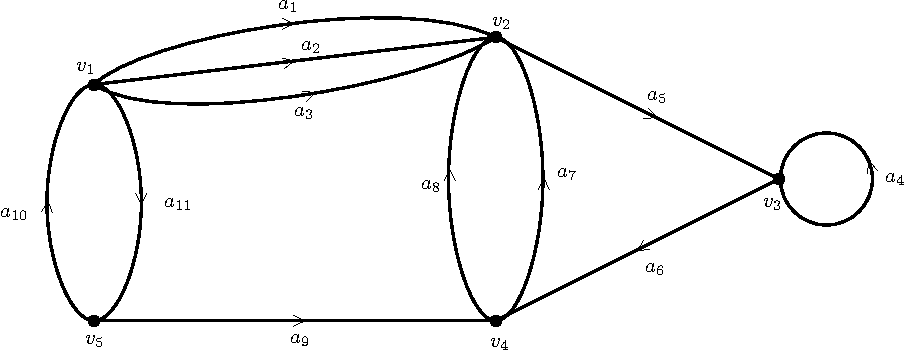
\includegraphics[scale=.9]{images/graph37.pdf}
\caption{A directed graph on $5$ vertices.}
\end{figure}
\end{exmp}
\begin{defn} Let $G=(V,A)$ be a directed graph. Let us note $V(G)=\{v_1, \dots ,  v_n\}$. The \textbf{adjacency matrix} of $G$, is the matrix $M=(m_{ij})_{1 \leq i,j \leq n }$ where $m_{ij}$ is the number of edges $e$ such that $\varphi(e)=(u_i,v_j)$.
\end{defn}
\begin{exmp} The adjacency matrix of the above graph is given by:
\begin{align*}
M=\begin{pmatrix}
0 & 2 & 0 & 0 & 1 \\
1 & 0 & 1 & 0 & 0 \\
0 & 0 & 1 & 0 & 0 \\
0 & 2 & 1 & 0 & 0 \\
1 & 0 & 0 & 1 & 0
\end{pmatrix}.
\end{align*}
\end{exmp}
\begin{defn} The definitions of walks, trails, paths, cycles, circuits, etc. can be obviously adapted. The \textbf{in-degree} of a vertex of a directed graph, denoted by $v^-$, is the number of edges that end at that vertex. The \textbf{out-degree} of a vertex, denoted by $d^+$, is the number of edges that start at that vertex. A directed graph is called \textbf{balanced} if for each vertex $v$ of the graph, we have $d^+(v)=d^-(v)$.
\end{defn}
\newpage
\begin{prop} Let $G=(V,A)$ be a directed graph with adjacency matrix $M=(m_{ij})$, then:
\begin{align*}
|A(G)| = \sum_{v \in V} d^+(v) = \sum_{v \in V} d^-(v) = \sum_{i,j=1}^n m_{ij}.
\end{align*}
\end{prop}
\begin{proof}
Follows from the following simple remarks: 
\begin{align*}
&d^+(v_i) = \sum_{j=1}^n m_{ij} \implies \sum_{i=1}^n d^+ (v_i)= \sum_{i=1}^n \sum_{j=1}^n m_{ij}. \\
&d^-(v_j)= \sum_{i=1}^n a_{ij} \text{ and } \sum_{j=1}^n \sum_{i=1}^n d^-(v_j)= \sum_{j=1}^n \sum_{i=1}^n m_{ij}. 
\end{align*}
\end{proof}
\begin{defn} A directed graph $G$ is called \textbf{strongly connected} if for all $(u,v) \in V(G)^2$, there exists a path from $u$ to $v$.
\end{defn}
\begin{rem} Define $u \sim v$ iff there exists $(u,v)$-path and therte exists a $(v,u)$-path. Then $\sim$ is an equivalence relation. 
\end{rem}
\begin{thm} A directed graph $G$ has a closed Euclidian trail iff it is balanced and strongly connected. 
\end{thm}
\begin{proof}
First we prove that the conditions are necessary. As a closed Eulerian trail leaves each vertex as many times as it enters it, $G$ must be balanced. Similarly we have a trail from any vertex to any vertex implies that $G$ is strongly connected. To see that these conditions are sufficient, we copy the proof of the wanted case by replacing edges with directed edges. 
\end{proof}
\begin{defn}If we direct each edge of a complete graph on $n$ vertices, then the resulting directed graph is called a \textbf{tournament}.
\end{defn}
\begin{thm} All tournaments have a Hamiltonian path. 
\end{thm}
\begin{proof}[First proof]
Let us prove the claim by induction on $n$, the number of vertices of a tournament $T$. If $n=2$, then the statement is obvious. Now assume that we know the statement is true for all tournament having $n-1$ vertices. Let $T$ be any tournament on $n$ vertices. Let $v$ be any vertex. Let $T'=T-v$. By the induction hypothesis $T'$ has a Hamiltonian path $h=h_1h_2 \dots h_{n-1}.$ If thre is an index $i$ such that $h_iv$ is an edge and $vh_{i+i}$ is an edge, then we insert $v$ between $h_i$ and $h_{i+1}$. If If no such edge exists then there must exist an index $k$ such that $0 \leq k \leq n-1$ and $vh_j$ is an edge and for all $j>k$, $h_j v$ is an edge. Therefore either $vh_j$ is an edge or $h_{n-1}v$ is an edge. So we can fix $v$ either to the front of the end of $h$. 
\end{proof}
\newpage
\begin{proof}[Second proof] Let $C=(v_0, \dots ,  v_q)$ be a path of maximal length in $T=(V,A)$ and let us assume that there exists $v \in V$ such that $v \notin C$. Since $C$ is maximal $(v,v_0) \notin A$ and thus $(v_0,v) \in A$. Similarly we have $(v,v_q) \in A$. Let $i$ be the smallest index such that $(v,v_i) \in A$. Then $i>0$. Let us then replace $(v_{i-1},v_i)$ by $(v_{i-1},v_1v_i)$. We then have a path which is longer then $C$,  thus a contradiction. Consequently $C$ is a Hamiltonian path. 
\end{proof}
\begin{defn} A tournament $T=(V,A)$ is called \textbf{transitive} if for $(u,v) \in A$ and $(v,w) \in A$ we also have $(u,w) \in A$.  
\end{defn}
\begin{prop} A tournament is transitive iff it does not contain  a closed trail (circuit).
\end{prop}
\begin{proof}
"$\implies$" Assume that $T$ is transitive and has a circuit $C=(v_1,v_2, \dots , v_n,v_1)$. We have for $(v_1,v_2) \in A$ and $(v_2,v_3) \in A$ also that $(v_1,v_3) \in A$. Continuing we see that $(v_1,v_n) \in A$, which is not possible because $(v_n,v_1)$ is  in $A$ already. \\
"$\Longleftarrow$" Let $(u,v) \in A$ and $(u,w) \in A$ for a tournament $T$. Since $T$ does not have a cycle $(w, u) \notin A$. Hence $(u,w) \in A$. 
\end{proof}
\begin{thm} Let $T$ be a tournament which is strongly connected, with $|T| \geq 3$. Let $v \in V(T)$, then for all $k \in \{3, \dots , n\}$, $T$ contains a circuit of length $k$ which also contains $v$. 
\end{thm}
\begin{proof}
Let $v \in V(T)$. We prove this result with an induction on $k$. Let $k=3$. We note $V^+(v)$, the set of successors of $v$ and $V^-(v)$ the set of predecessors of $v$. We have $V^+ \cap V^- = \emptyset$ and $V^+ \neq \emptyset$, $V^- \neq \emptyset$ because $T$ is a strongly connected tournament. There exists an edge $(w,w') \in A$, with $w \in V^+$ and $w \in V^-$. We obtain a circuit of length $3$ by connecting $(v,w,w')$ which contains $v$. \\\\
Let us assume that the result is established for $k \in \{ 3, \dots , n-1\}$ and let us prove it for $k+1$. Let $C= (v_0,v_1, \dots ,  v_k=v_0)$ be a circuit of length $k$ that contains $v$. There exists a vertex of $T$ that is not in $V$. Then we distinguish between two cases: \\\\
\textbf{Case 1:} There exists $u \in V(T) \setminus V(C)$ and $i,j \in \{1, \dots k\}$ with $i \neq j$ such that $(v_i,u) \in A, (u,v_j) \in A$. Without loss of generality, we may take $i=1$. Then $(v_1,u) \in A$ and $(v_j,u) \notin A$. Hence the set $\{h \in \{1,  \dots , j-1\} \mid (v_h,u) \in A \}$ has a greatest element $h_0$. We deduce that $(v_{h_0},u) \in A, (v_{h_0-1},u) \notin A$ and that $(u,v_{h_0 +1}) \in A$. We replace $(v_{h_0},v_{h_0-1})$ with  $(v_{h_0}, u,v_{h_0-1})$ and we obtain a new circuit of length $k+1$. 
\newpage
\noindent \textbf{Case 2:} For all $u \in V(T) \setminus V(C)$, either $(u,v_i) \in A$ for all $i \in \{1, \dots ,  k\}$ or $(v_i,u) \in A$ for all $i \in \{1, \dots , k\}$. Consider the sets:
\begin{align*}
R&= \{ u \in V(T) \setminus V(C) : \forall i \in \{1, \dots , k \}, \ (u,v_i) \in A \} \\
S&= \{ u \in V(T) \setminus V(C) : \forall i \in \{1, \dots ,  k \}, \ (v_i,u) \in A\}.
\end{align*}
As $T$ is strongly connected, $R \neq \emptyset$ and $S \neq \emptyset$, and there exists $r \in R, s \in S$ with $(s,r) \in A$. We then replace $(v_0,v_1,v_2)$ with $(v_0,s,r,v_2)$ and we obtain a circuit of length $k+1$.
\end{proof}
\newpage
\section{Matchings}
\begin{defn} Let $G=(V,E)$ be a simple graph. A subset $M \subset E$ of edges is called a \textbf{matching} if no pair of edges shares a common vertex. Given a matching $M$ in a graph $G$, the vertices belonging to the edges of $M$ are said to be \textbf{saturated} by $M$ (or $M$-saturated). The other vertices are $M$-unsaturated. If $M$ saturates every vertex of $G$, then $M$ is said to be a \textbf{perfect matching}.
\end{defn}
\begin{exmp} \
\begin{enumerate} 
\item \  \begin{figure}[hbtp]
\centering
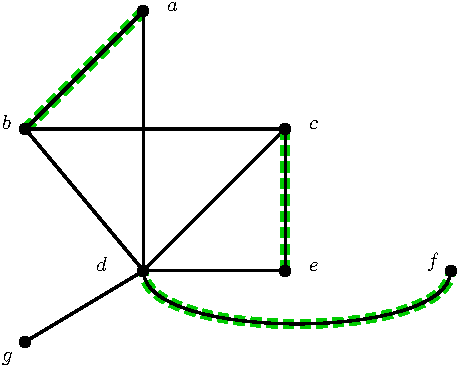
\includegraphics[scale=.9]{images/graph38.pdf}
\caption{See description below.}
\end{figure} \\
$M_1= \{ab,ce,df\}$ is a matching (depicted in green in the above figure). Moreover, $M_2=\{cd,ab\}$ is also a matching, $M_3= \{df\}$ is a matching. $a,b,c,d$ are $M_2$-saturated and $e,f,g$ are $M_2$-unsaturated. The only $M_1$-unsaturated vertex is $g$. 
\item \
\begin{figure}[hbtp]
\centering
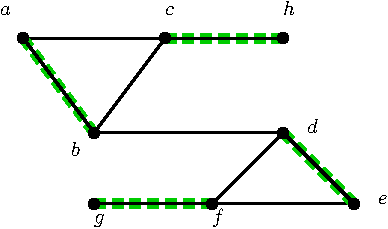
\includegraphics[scale=.9]{images/graph39.pdf}
\caption{See description below.}
\end{figure}
\\ $M= \{ab,ch,de,fg\}$ is a perfect matching. 
\end{enumerate}
\end{exmp}
\newpage
\begin{defn} A \textbf{maximum matching} in a graph is a matching that has the largest possible cardinality. We denote the cardinality of a maximal matching as $\nu(G)$. A \textbf{minimal matching} is a matching that cannot be enlarged by addition of an edge. 
\end{defn}
\begin{exmp} \
\begin{figure}[hbtp]
\centering
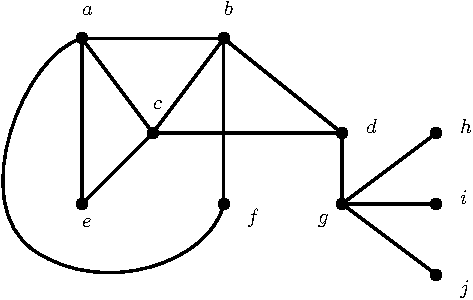
\includegraphics[scale=.9]{images/graph41.pdf}
\caption{Depiction of maximal matchings.}
\end{figure}
\\
$M_1=\{ae,bf,cd,gh\}$ is a maximum matching. $M_2=\{dg,af,bc\}$ is a maximal matching but not a minimal. 
\end{exmp}
\begin{defn} Given a matching $M$, an $M$-\textbf{alternating path} in $G$ is a path where the path alternates between $M$-edges and non $M$-edges. An $M$-\textbf{augmenting path} is an $M$-alternating path whose both end vertices are $M$-unsaturated. 
\end{defn}
\begin{exmp} \ 
\begin{figure}[hbtp]
\centering
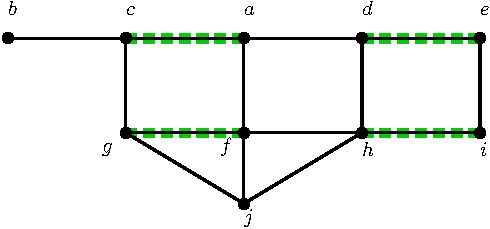
\includegraphics[scale=.9]{images/graph42.pdf}
\caption{$M$-alternating path and $M$-augmenting path.}
\end{figure}
\\
$c,a,d,e,i$ is an $M$-alternating path, whereas $j,g,f,a,c,b$ is an $M$-augmenting path. 
\end{exmp}
\newpage
\begin{thm}[Berge] Let $M$ be a matching in a graph $G$. $M$ is maximal iff $G$ contains no $M$-augmenting paths. 
\end{thm}
\begin{proof}
First assume that $M$ is a maximum matching, and suppose that $P=v_1v_2, \dots , v_k$ is an $M$-augmenting path. Then it must be even and the edges $v_2v3,v_4v_5,\dots,v_{k-2}v_{k-1}$ are edges of $M$, while $v1v_2,v_3,v_4, \dots ,  v_{k-1}v_k$ are not edges of $M$. 
\\
\begin{figure}[hbtp]
\centering
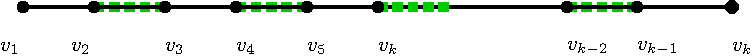
\includegraphics[scale=.9]{images/graph43.pdf}
\caption{The situation as described above.}
\end{figure}
\\
But then if we define $M_1$ to be:
\begin{align*}
M_1:= ( M \setminus \{ v_2v_3, \dots , v_{k-2}v_{k-1}\} ) \bigcup \{ v_1v_2, \dots , v_{k-1}v_k\},
\end{align*}
then $M_1$ is a matching that contains one more edge than $M$. This is a contradiction and hence $G$ contains augmenting paths. 
\\\\
For the converse, assume that $G$ has no $M$-augmenting paths, and suppose that $M'$ is a matching that is larger than $M$. We define a subgraph $H$ of $G$ as follows: $V(G)=V(H)$ and $E(H)= M \Delta M'= (M' \setminus M) \cup (M \setminus M')$. Since each of the vertices of $G$ has at most one edge from $M$ and at most one edge from $M'$ it follows that $\Delta(H) \leq 2$. This implies that each connected component of $H$ is either a single vertex, a path, or a cycle. If a component is a cycle, then it must be an even cycle, since the edges alternate between $M$-edges and $M'$-edges. Since $|M'| >|M|$ there must be at least one component of $H$ that is a path that begins and ends on the edges from $M'$. But this is an $M$-augmenting path, which is a contradiction. Therefore no such matching $M'$ can exist and $M$ is maximal. 
\end{proof}
\newpage
\begin{defn} If $G$ is a bipartite graph. $G=(X,Y;E)$, we say that $X$ can be \textbf{matched into} $Y$ if there exists a matching in $G$ that saturates the vertices of $X$. A set $T$ of vertices in a graph $G$ is said to \textbf{cover} the edges of $G$ if every edge of $G$ is incident with at least one vertex of $T$. Such a set $T$ is called an \textbf{edge cover} of $G$.
\end{defn}
\begin{exmp} \
\begin{figure}[hbtp]
\centering
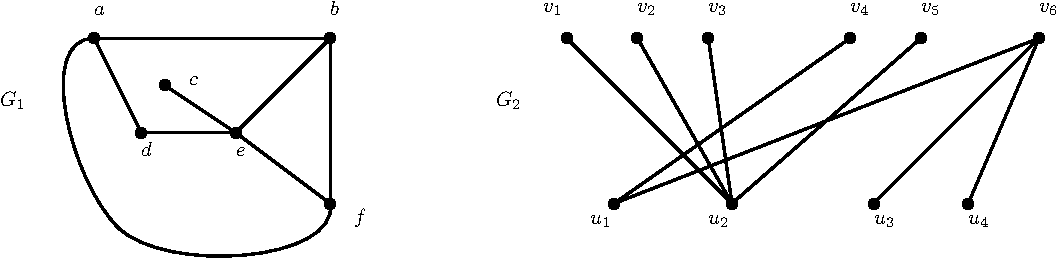
\includegraphics[scale=.65]{images/graph44.pdf}
\caption{Two edge covers.}
\end{figure}
\\
In $G_1$, the set $\{b,d,e,a\}$ is an edge cover, as is the set $\{a,e,f\}.$ In $G_2$, $\{v_1,v_2,v_3,v_4,v_5,v_6\}$ is an edge cover as is the set $\{v_2,v_6,v_1\}.$
\end{exmp}
What is the size of a minimum edge cover? We note $\tau (G)$ the size of a minimum edge cover. 
\begin{lem}\label{prevlemma} Recall that for a graph $G$, $\nu(G)$ is the size of a maximal matching and $\tau(G)$ is the size of a minimum edge cover. We have $
\nu(G) \leq \tau(G)$. 

\end{lem}
\begin{proof}
An edge cover $T$ contains one end vertex at least of each edge $e$ of a matching $M$ in $G$. To each edge $e$ of $M$, we can associate one of its endpoints $v_e$. As $M$ is a matching for $e \neq f$, $v_e \neq v_f$. We thus have \begin{align*}
|T| \geq | \{v_e : e \in M \} | = |M|.
\end{align*}
Since this is true for any edge cover $T$ and any matching $M$ it follows that 
$\tau(G) \geq \nu(G).$

\end{proof}
\begin{exmp} \
\begin{figure}[hbtp]
\centering
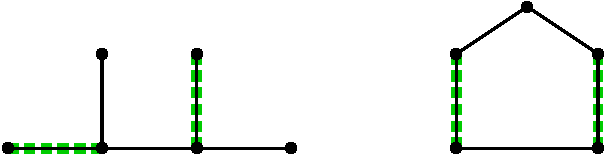
\includegraphics[scale=.65]{images/graph45.pdf}
\caption{See Lemma above.}
\end{figure}
\end{exmp}
\newpage
\begin{thm}[König-Egerváry] Let $G=(U,V;E)$ be a bipartite graph. We have $\tau(G)=\nu(G)$. 
\end{thm}
\begin{proof}
Let $M$ be a maximum matching of $G=(U,V;E)$. For $X \subset V(G)$, we note $N_M(X)$ the neighbors of elements in $X$, in the subgraph $(U,V;M)$. We partition $U$ as $U_1 \cup U_2 \cup U_3$ and $V=V_1 \cup V_2 \cup V_3$ as follows: 
\begin{align*}
U_1 &= \{u \in U : u \text{ is not } M\text{-saturated}\}. \\
V_1 &= \{v \in V : v \text{is not } M\text{-saturated}\}. \\
U_2 &=\{ u \in U \setminus U_1 : \exists u' \in V_1 \text{ and a } (u',u)-\text{path which is $M$-saturated}\}. \\
V_2 &= N_M(U_2). \\
U_3 &= U \setminus (U_1 \bigcup U_2). \\
V_3 & = N_M(U_3). 
\end{align*}
\
\begin{figure}[hbtp]
\centering
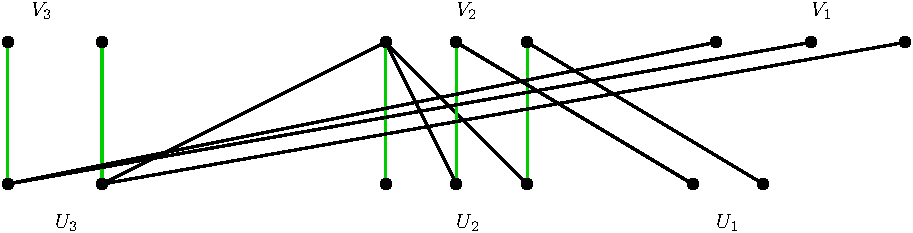
\includegraphics[scale=.85]{images/graph46.pdf}
\caption{The partition of $U$ and $V$.}
\end{figure}
\\
We first show that $Q=U_3 \cup V_2$ is a edge cover. If $Q$ were not an edge cover, then there would exist an edge $\{u,v\}$, with $u \in U_1 \cup U_2$ and $v \in V_3 \cup V_2$.  If $u \in U_2$, we note $P_u$ a path from $u' \in V_1$ to $u$. If $u \in U_1$., we just note $P_u$ to the empty walk $(u)$. 
\\\\
\textbf{Case 1:} $v \in V_1$. In this case $P'=P_u \cup \{u,v\}$ would be $M$-augmenting and Berge's theorem implies that $M$ is not maximal, which is a contradiction.
\\\\
\textbf{Case 2:} $v \in V_3$. Let $v_m \in N_M(v)$, $P'= P_u \cup \{u,v\} \cup \{v,v_m\}$. Then $(v',v_m)$ would be $M$-alternating, $u' \in V_1$, we have $v_m$ should be in $U_2$ and not in $V_3$. Contradiction. 
\\\\
Thus $Q$ is an edge covering of $G$. Next we note that $|V_2| = |N_M(U_2)|=|U_2|$. Hence $|Q|=|V_2 \cup U_3| = |V_2| + |U_3| = |U_2| + |V_3|=|M|.$ Now, using the previous lemma (Lemma \ref{prevlemma}), we see that $|M| \leq \nu(G) \leq \tau(G) \leq |Q|= |M|$ and thus $\nu(G)= \tau(G)$. 
\end{proof}
\newpage
We now state a result that is not necessarily graph theoretical. 
\begin{defn} Let $\mathcal{A}= (A_i)_{i \in I}$ be a family of non empty sets. Let $S= cup_{i \in I} A_i$. A \textbf{system of representations} of the family $\mathcal{A}$, noted \textbf{SR}, is a family of elements $(x_i)_{i \in I}$ of $S$,  such that $x_i \in A_i$ for all $i \in I$. A \textbf{system of distinct representations} of the family $\mathcal{A}$, noted \textbf{SDR}, is a family $(x_i)_{i \in I}$ of SR, such that $x_i \neq x_j$ if $i \neq j$. 
\end{defn}
\begin{exmp} $A_1=\{2,8\}$, $A_2=\{8\}$, $A_3=\{5,7\},$ $A_4=\{2,4,8\}$, $A_5=\{2,4\}$. The family $\mathcal{A}= (A_i)_{i=1}^5$, has a SDR, namely $\{2,8,7,4\}$. The family $\mathcal{A}'=(A_1,A_2,A_4,A_5)$ does not have a SDR.
\end{exmp}
\begin{thm}[Hall] A finite family $\mathcal{A}=(A_i)_{i \in I}$ of non empty sets has a SDR iff $\mathcal{A}$ satisfies Hall's property: 
\begin{align*}
\forall J \subset I, \ |A_J| = \left| \bigcup_{i \in J} A_i \right| \geq |J|.
\end{align*}
\end{thm}
\begin{proof} For all $J \subset I$, we note $A_J= \cup_{i \in J} A_i$. \\
"$\implies$" Let us assume that the family $\mathcal{A}$ has a SDR $(x_i)_{i \in I}$. For $J \subset I$, $A_J$ contains $\{x_i, i \in J\}$ which is by definition  of cardinality $J$, thus $|A_J| \geq |J|$. 
\\\\
"$\Longleftarrow$" Let us now assume that $\forall J \subset I$, $|A_J| \geq |J|$.  \\
If for each $i \in I$, $A_i = \{x_i\}$, then $(x_i)_{i \in I}$ is a SDR. Otherwise, $\exists i_0 \in I$ such that $A_{i_0}$ contains at least two distinct elements $x$ and $y$. Let $B_{i_0} = A_{i_0} \setminus \{x\}$ and $C_{i_0} = A_{i_0} \setminus \{y\}$. Let $\mathcal{B}$ and $\mathcal{C}$ be the families obtained by replacing $A_{i_0}$ with respoectively $B_{i_0}$ and $C_{i_0}$. We next show that one of $\mathcal{B}$ and $\mathcal{C}$ satisfies Hall's criterion. 
\\\\
If not, there would exists $J$ and $M$ in $I \setminus \{i_0\}$, such that 
\begin{align*}
|J \cup \{i_0\} | > |B_{i_0} \cup A_J| \implies |J| \geq |B_{i_0} \cup A_J|,
\end{align*}
and
\begin{align*}
|K| \geq |C_{i_0} \cup A_J|.
\end{align*}
Note $S= B_{i_0} \cup A_J$, $T= C_{i_0} \cup A_M$. We thus have $J|  \geq |S| + |M| \geq |T|$. But $S \cup T= B_{i_0} \cup C_{i_0} \cup A_J \cup A_M = A_{i_0} \cup A_{J \cup M}$, and it follows from Hall's condition that $|S \cup T \| \geq 1 + |J \cup M|$.  
\\\\
Moreover $S\cap T = (B_{i_0} \cup A_J) \cup (C_{i_0} \cup A_M) = A_J \cap A_M$. Hence it follows again from Hall's condition that $|S \cap T| \geq  |J \cap M|$. Consequently $|J| + |M| \geq |S| + |M| = |S \cup T| + |S \cap T| \geq 1 + |J \cup M| + |J \cap M| = 1 + |J| + |M|,$ which is a contradiction. Thus either $\mathcal{B}$ or $\mathcal{C}$ satisfies Hall's condition. The set $I$ being finite, representing the process we obtain a family of sets with one element satisfying Hall's condition. Such a family is a SDR for $\mathcal{A}$. 
\end{proof}
Now we give a graph version of Hall's theorem.
\begin{thm} Let $G=(A,B;E)$ be a bipartite graph. Then $G$ has a perfect matching iff 
\begin{enumerate}
\item $|A|=|B|$.
\item For all $X \subset A, \ |N(X)| \geq |X|$. 
\end{enumerate}
\end{thm}
\begin{proof}
"$\implies$" If $G$ has a perfect matching $M$, then for all $X \subset A$, $|N(X)| \geq |N_M(X)|=|X|$. In particular $|A|=|N_M(A)|=|B|$. \\
"$\Longleftarrow$" Let $Q$ be an edge cover of minimal cardinality. Let $A_1= Q \cap A$, $B_1=Q \cap B$ and $A_2=A \setminus A_1$. As $Q$ is an edge cover we have $N(A_2) \subset B_1$ and so $|B_1| \geq |N(A_2)| \geq |A_2|$. By the König-Egerváry theorem, we obtain that
\begin{align*}
\nu(G)=\tau(G)=|Q|=|A_1 \cup B_1| = |A_1| + |B_1| \geq |A_1| + |A_2| = |A|.
\end{align*}
We have then proven that $G$ has a matching $M$ for which all vertices of $A$ are saturated. So $|A| < |B|$ and $M$ is a perfect matching. 
\end{proof}
\begin{cor} A bipartite regular graph admits a perfect matching.
\end{cor}
\begin{proof}
Let $G=(A,B;E)$ be bipartite and $k$-regular. For all $X \subset A$, we have 
\begin{align*}
k|X|= \sum_{u \in X} d(u) = E|G[X \cup N(X)]|  \leq \sum_{v \in N(X)} d(v) = k |N(X)|,
\end{align*}
thus $|X| \leq |N(X)|$ for all $ X \subset A$. Similarly we show for all $X \subset B$ that $|X| \leq N(X)|$. Take then $X=A$ and $B$ to obtain $|A|=|B|$. 
\end{proof}
As an application we study the marriage problem. Let us consider a set of 5 boys $\{b_1, \dots , b_5\}$ and a set of $5$ girls $\{g_1, \dots , g_5\}$. Each boy $g_i$ makes  a list of his favourite girls. 
\begin{align*}
b_1=\{g_1,g_2,g_3\}, \ b_2=\{g_4,g_5\}, \ b_3=\{g_4\}, \ b_4=\{g_5\}, \ b_5=\{g_2,g_5\}.
\end{align*}
Is it possible that each boy can marry one of his favourite girls?. Let $G=(A,B;E)$. $A=\{b_1, \dots ,  b_5\}$, $B=\{g_1, \dots , g_5\}$ and $\{b_i,g_i\}$ is an ?? iff $g_i$ is on the list of favourite girls of $b_i$. The problem has a solution iff $G$ has a perfect matching. But for $A'=\{b_2,b_3,b_4\}, \ N(A')=\{g_4,g_5\}$ and $|A'| > |N(A')|$ so there is no perfect matching. There also exists a necessary and sufficient condition for the existence of perfect matching for a generic graph. If $G$ is a graph and $S \subset V(G)$ then we denote $c_0(G-S)$ the number of connected components of $G-S$ that have an odd number of vertices. 
\begin{thm}[Tutte's theorem] A graph $G$ has a perfect matching iff for all subsets $S$ of the vertex set of $G$, we have $c_0(G-S) \leq |S|$. 
\end{thm}
\newpage
\section{Planar graphs}
\begin{defn} Let $G$ be a graph that can be drawn on a plane surface so that no of its edges intersect. Then $G$ is called a \textbf{planar graph}. Let $G$ be a planar graph. Then the edges of $G$ partition the plane into regions,  we will call these regions the \textbf{faces} of $G$. 
\end{defn}
\begin{exmp} \
\begin{figure}[hbtp]
\centering
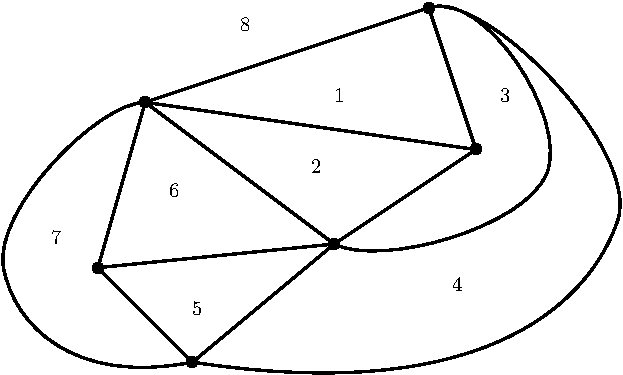
\includegraphics[scale=.9]{images/graph47.pdf}
\caption{Example of a planar graph as defined above.}
\end{figure}
\end{exmp}
\begin{thm}[Euler's theorem on Planar graphs] Let $G$ be a connected planar graph with $V$ vertices, $E$ edges and $F$ faces. Then 
\begin{align*}
V+F=E+2.
\end{align*}
\end{thm}
\begin{proof}
We prove the statement by induction on $E$, the number of edges of $G$. If $E=1$, then $G$ is either a tree of one edge, $V=2,F=1$, and the statement is true, or $G$ is the one vertex graph with a loop, thus $V=1, F=2$, and the statement is true again. \\\\
$E-1 \to E$. Assume that $G$ has $E$ edges. We distinguish two cases. If we can omit an edge $e$ from $G$ so that the new graph $G'$ is still connected, then $e$ is in a cycle in $G$, and therefore from  ???? his faces on the two sides of $e$ in $G$. Then $G'$ has $E-1$ edges, $V$ vertices and $F_1$ faces. Therefore $V+F-1=E-1+2$ which gives $V+F=E+2$. If there is no $e$ with the mentioned property, then $G$ is a cycle-free connected graph, that is a tree. Then $V=E+1$. On the other hand $F=1$ So the claim is true. 
\end{proof}
\newpage
\begin{exmp} The graph $K_{3,3}$ is not planar.
\end{exmp}
\begin{rem}The previous definitions and results are intuitively \textit{simple}, but we need to define them more rigorously.
\end{rem}
\begin{defn} A graph $G$ is called planar if it has a representation in $\mathbb{R}^2$ in such a way that its edges are \textbf{simple curves} which do not intersect except at their endpoints. So in a planar graph the edges can intersect only at vertices. 
\end{defn}
\begin{rem} Note that a planar representation of a graph is not unique in general. 
\end{rem}
\begin{exmp} \
\begin{figure}[hbtp]
\centering
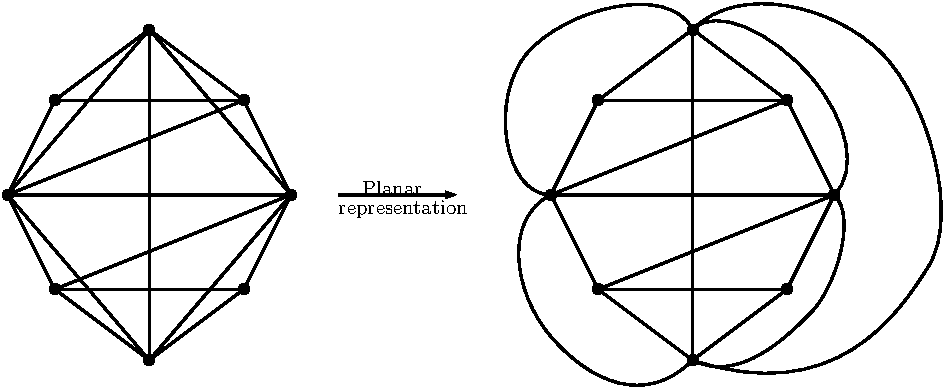
\includegraphics[scale=.8]{images/graph48.pdf}
\caption{Example of a planar graph as defined above.}
\end{figure}
\end{exmp}
We shall use in what follows \textbf{Jordan's theorem}: A simple closed curve splits the plane in two domains (that is an open and connected set  in $\mathbb{R}^2$), one of them being bounded and the other is unbounded. The curve is the common boundary to these two domains. In the representation of a planar graph $G$, the complements of edges given a partiton of the plane $\mathbb{R}^2$ into domains, called the faces of the graph $G$. By definition,  a planar representation of a graph has one unbounded face,  which we shall call the \textbf{exterior face} or the \textbf{infinite face} of $G$. 
\\\\
A face $f$ of a connected graph has as boundary a closed walk called the boundary of $f$. The length of the face $f$ is noted $l(f)$ and is the length of this closed walk. \newpage
\begin{exmp} \
\begin{figure}[hbtp]
\centering
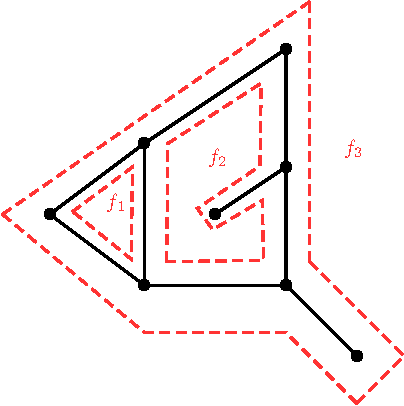
\includegraphics[scale=.9]{images/graph49.pdf}
\caption{Three faces $f_1,f_2,f_3,$ with $l(f_1)=3, \ l(f_2)=7, \ l(f_3)=8$.}
\end{figure}
\end{exmp}
\begin{rem}A forest is a planar graph with a single face (the infinite face). 
\end{rem}
\begin{exmp} The graph $K_{3,3}$ is not planar. Indeed, suppose that $K_{3,3}$ has a planar representation. If $\{a_1,a_2,a_3\} \cup \{b_1,b_2,b_3\}$ is the partition of $V(K_{3,3})$, let $(a_1, b_1,a_2,b_2,a_1)$ be the $4$-cycle of $K_{3,3}$. It follows from the Jordan's theorem that $C$ partitions the plane into two domains. If $b_3$ is inside (resp. outside $C$), $a_3$ cannot be either inside, nor outside. 
\end{exmp}
\begin{exmp}$K_5$ is not planar. If $K_5$ had a planar representation, let $C$ be the $5$-cycle of $K_5$. It follows from Jordan's thereom that $C$ splits $\mathbb{R}^2$ into two domains. The $5$ diagonals of $C$ are edges of $K_5$. Among these $5$ diagonals,  at most 4 can be drawn inside $C$ and 2 outside $C$. Hence we cannot draw the last diagonal without crossing another diagonal. 
\end{exmp}
\begin{rem}
Euler's formula for connected graphs is $n-m+r=2$, where $n=|V|$, $m=|E|$, $r$ is the number of faces.
\end{rem}
As a consequence of Euler's formula we have:
\begin{cor} The number of faces of a planar graph does not depend on the chosen representation. 
\end{cor} 
\newpage
\begin{lem} Let $G=(V,E)$ be a planar graph. We note $F$ the set of its faces. We then have 
\begin{align*}
2|E|= \sum_{j \in F} l(f),
\end{align*}
where $l(f)$ is the length of the face $f$. 
\end{lem}
\begin{cor} Let $G$ be a simple planar graph, of order $n \geq 3$, with $|E|=m$. We have: 
\begin{align*}
m \leq 3n-6.
\end{align*}
if in addition $G$ does not contain a triangle, then 
\begin{align*}
m \leq 2n-4.
\end{align*}
\end{cor}
\begin{proof}
We can assume $G$ is connected (otherwise we add edges). We have
\begin{align*}
2m= \sum_{f \in F} l(f).
\end{align*}
Since $G$ is simple, and $n \geq 3$, we have $l(f) \geq 3$. Hence $2m \geq 3 |F| = 3(2-n+m)$ which gives $3n \geq m+6$. If $G$ does not have a triangle, then $2m \geq 4|F|=4(2-n+m)$ which gives $2n \geq m+4$.
\end{proof}
\begin{cor}\label{lastcor} A simple planar graph $G$ satisfies $\delta(G) \leq 5$. If in addition it does not contain a triangle, then $\delta(G) \leq 3$. 
\end{cor}
\begin{proof}
We can again assume that $G$ is connected. If $\delta(G) \geq 4$, then $2m \geq 6n$. But from the previous corollarly $3n-6 \geq m \geq 3n$ which is a contradiction. If $G$ does not have a triangle we have $2m \geq 4n$ and $2n-5 \geq m \geq 2n$ which is again a contradiction. 
\end{proof}
\begin{defn} A polyhedron is a solid in $\mathbb{R}^3$ whose boundary is a union of polygons, called faces. The faces intersect at vertices and the lines that join two vertices are called edges. A polyhedron is called \textbf{regular}, if all its faces are regular polygons, i.e.  all its faces have the same number of edges, all vertices are contained in the same number $d$ of edges ($d$ is called the degree of the polyhedron), all edges have the same length, all angles within the faces are equal, and all angles between the faces are equal. 
\end{defn}
\begin{exmp}The cube is a regular polyhedron. 
\end{exmp}
\newpage
In combinatorics, we discussed the conditions on the length of the edges, and the sign of angles, but we keep the graph theoretical conditions that each face is a cycle with $l$ edges and each vertex has degree $d$. We will show, using Euler's formula, that there are only $5$ regular and convex polyhedra. 
\begin{thm} Let $P$ be a convex polyhedron with $V$ vertices, $F$ faces and $E$ edges. Then $V+F-E=2$. 
\end{thm}
Next it is easy to see that in any convex polyhedra $V$,  $3F \leq 2E$ and $3V \leq 2E$. From Corollary \ref{lastcor} we have $E \leq 3V-6$. Similarly $E \leq 3F-6$. 
\begin{lem} All convex polyhedra have at least one face that has at most five edges.
\end{lem}
\begin{proof}
We know that $E \leq 3F-6$ and 
\begin{align*}
\sum_{i=1}^F f_i = 2E \leq 6F-12.
\end{align*}
Therefore if $f_i \geq 6 \; \forall i$,  $\sum_{i=1}^F f_i \geq 6F$, which is a contradiction.
\end{proof}
Similarly, we establish
\begin{lem} All convex polyhedra have at least one vertex that is contained in at most five edges. 
\end{lem}
The previous lemma shows that in regular polyhedra, the degree $d$ of each vertex can only be $3,4$ or $5$. Same thing for $l$. So there are $3\times3 = 9$ cases to check. Then one can show that:
\begin{enumerate}
\item $d=3, \ l=3, \ F=5, \ V=4$ which is a tetrahedron.
\item $d=3, \ l=4, \ F=6, \ V=8$ which is a cube.
\item $d=3, \ l=5, \ F=12, \ V = 20$ which is a dodecahedron.
\item $d=4, \ l=3,  F=8, \ E=12, \ V=6$ which is octahedron.
\item $d=5, \ l=3, \ F=20, \ E=30, \ V=12$ which is a icosahedron.
\end{enumerate}
\begin{thm} There are five regular polyhedra: The tetrahedron, the cube, the dodecahedron, the octahedron, the icosahedron. 
\end{thm}
\end{document}